\chapter{نمودارهای توالی طراحی}
({\color{red}  بهنگام‌سازی شد.})\\
({\color{red}  ‌توضیح: به علت تغییراتی که امکان دارد برای فاز بعد در مورد کلاس‌های طراحی رخ بدهد، در این سند تنها نمودارهای توالی بهنگام‌سازی شده‌اند و ممکن است در مواردی کلاس‌های طراحی که در این فصل موجود است، طبق آخرین تغییرات طراحی نباشد. پس از نهایی شدن کلاس‌های طراحی، کلاس‌های موجود در این فصل نیز بهنگام‌سازی و کامل خواهند شد.})

\newpage
\begin{landscape}
\section{اضافه کردن پروژه}
\begin{figure}[H]
	\centering
	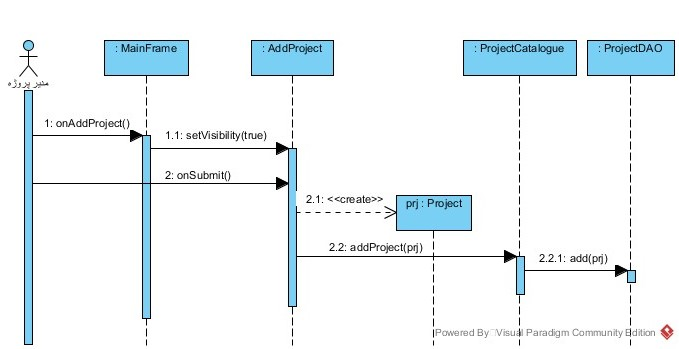
\includegraphics[scale=0.6]{img/sequence-design/AddProjectToOrganization}	
	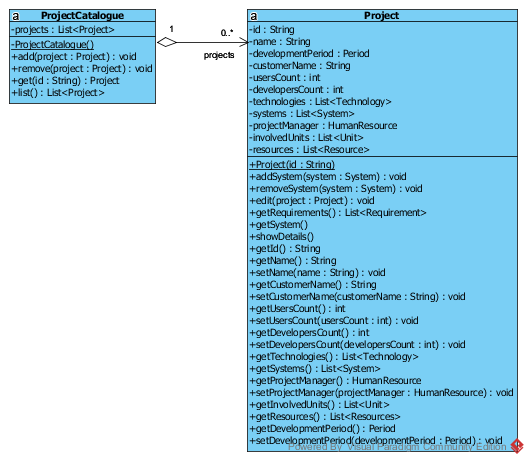
\includegraphics[scale=0.6]{img/sequence-design/AddProjectToOrganizationC}
	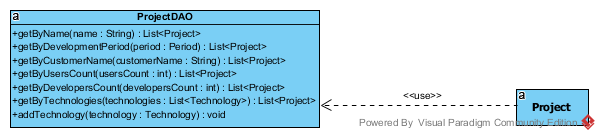
\includegraphics[scale=0.6]{img/sequence-design/AddProjectToOrganizationD}
	\caption{اضافه کردن پروژه}
\end{figure}
\end{landscape}

\begin{landscape}
\section{اضافه کردن سیستم به پروژه}
\begin{figure}[H]
	\centering
	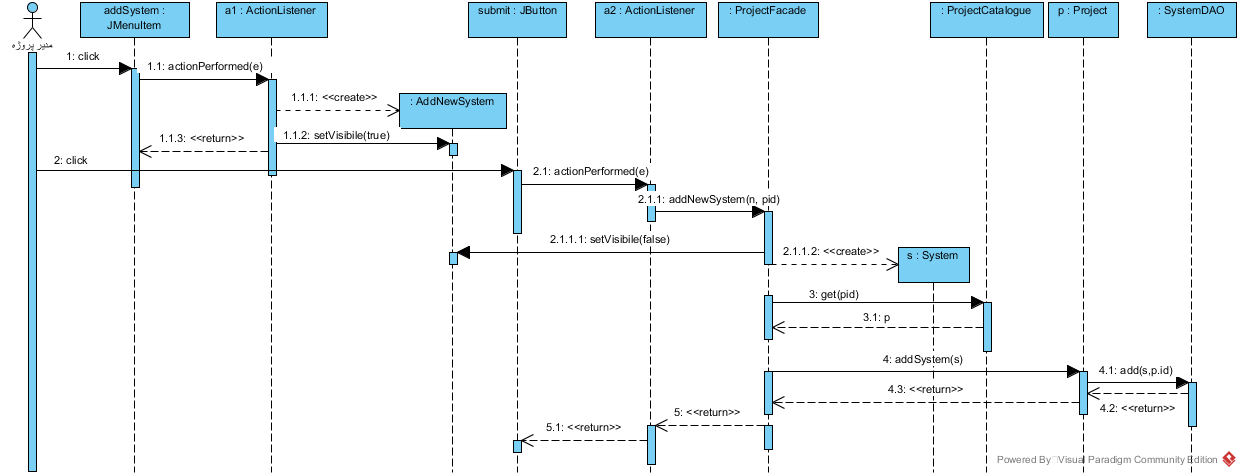
\includegraphics[scale=0.55]{img/sequence-design/AddSystemToProject}
	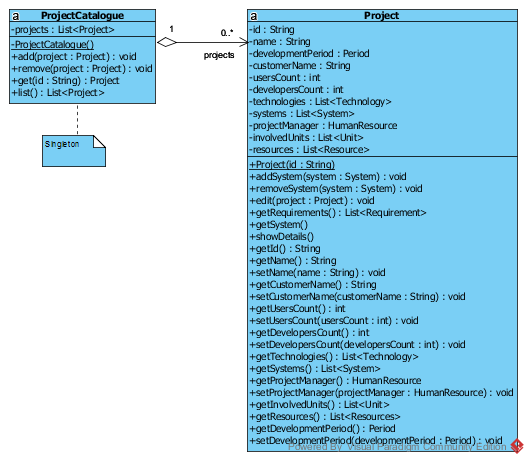
\includegraphics[scale=0.6]{img/sequence-design/AddSystemToProjectC}
	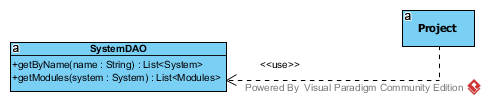
\includegraphics[scale=0.6]{img/sequence-design/AddSystemToProjectD}
	\caption{اضافه کردن سیستم به پروژه}
\end{figure}
\end{landscape}

\begin{landscape}
\section{اضافه کردن ماژول به سیستم}
\begin{figure}[H]
	\centering
	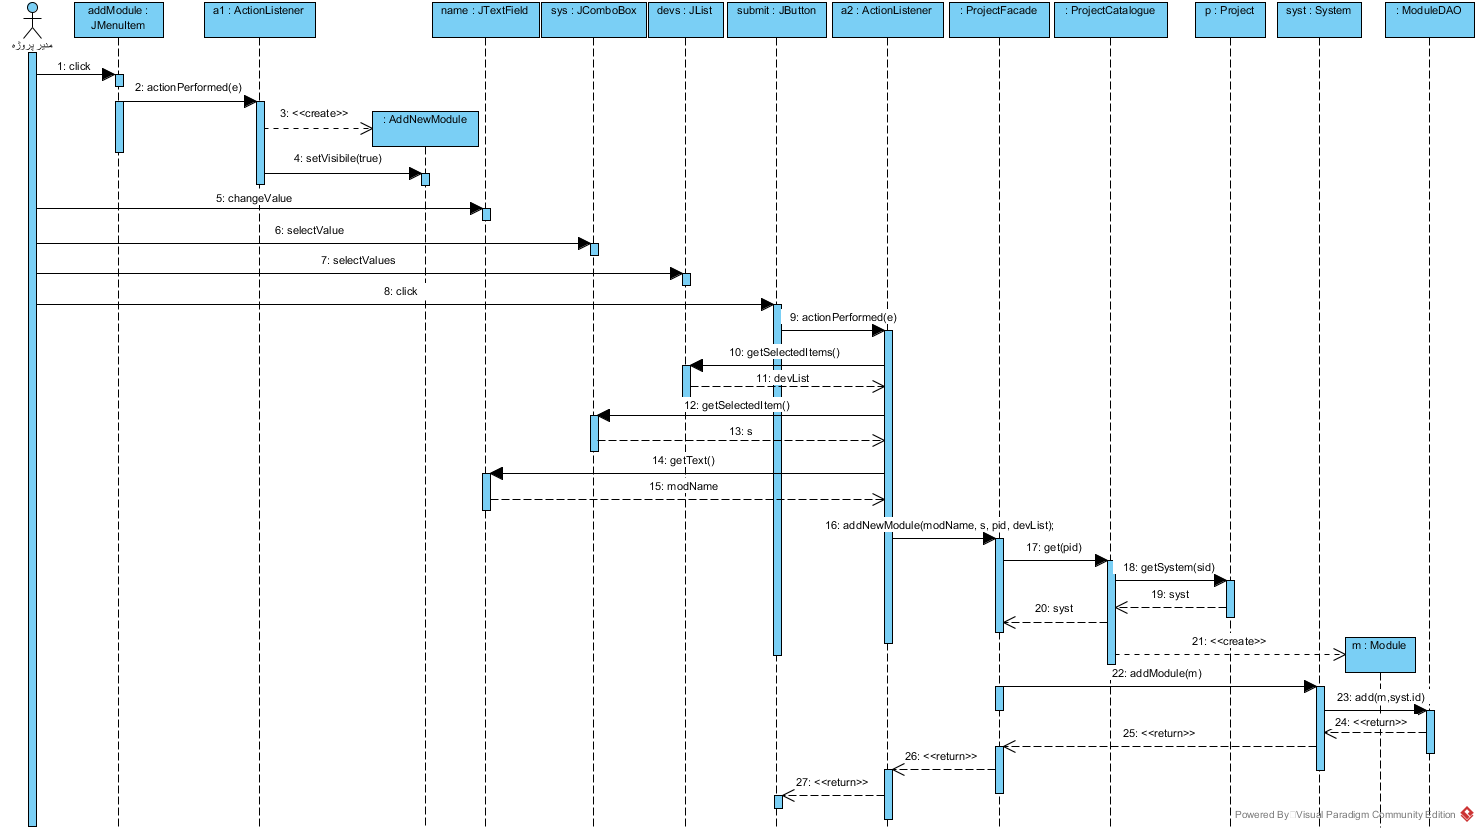
\includegraphics[scale=0.55]{img/sequence-design/AddModuleToSystem}
\end{figure}
\begin{figure}[H]
	\centering
	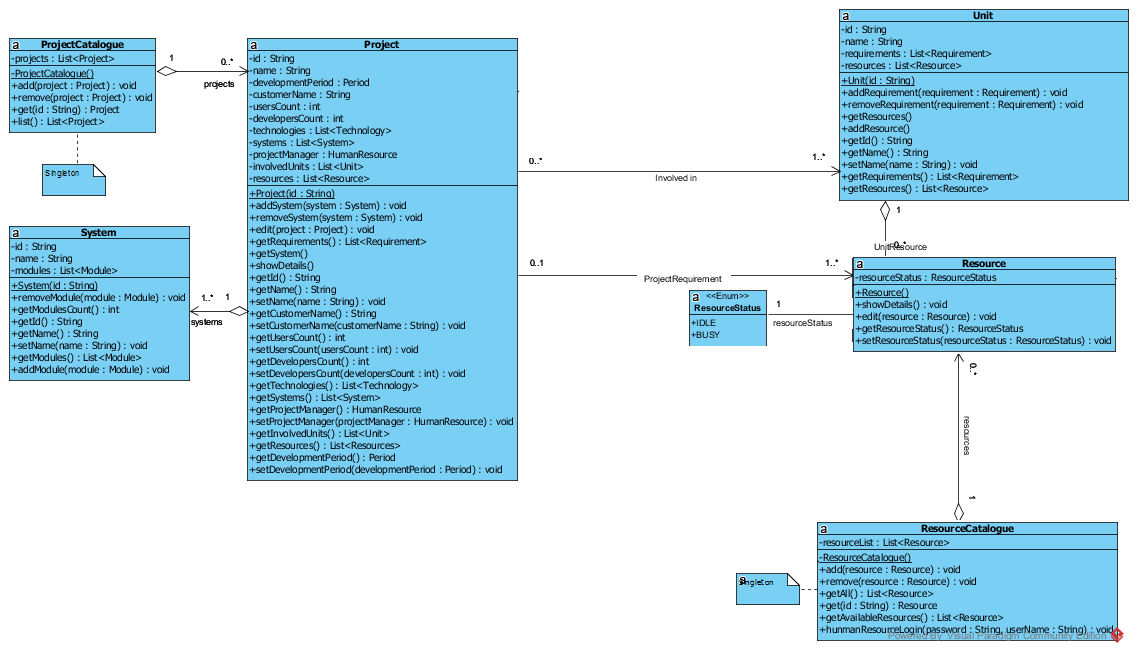
\includegraphics[scale=0.65]{img/sequence-design/AddModuleToSystemC}
	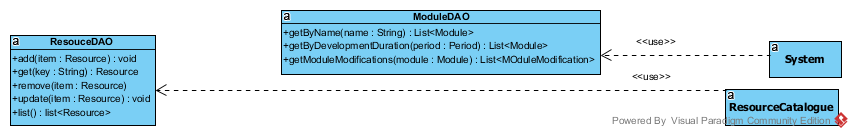
\includegraphics[scale=0.65]{img/sequence-design/AddModuleToSystemD}
	\caption{اضافه کردن ماژول به سیستم}
\end{figure}
\end{landscape}


\begin{landscape}
\section{اضافه کردن منبع به واحد سازمان}
این نمودار توالی به علت کلاس‌های زیادی که در آن درگیر هستند، در چهار تصویر و به این صورت در مستند آورده شده که در هر تصویر، تنها یک operand به صورت کامل نشان داده شده است.
\begin{figure}[H]
	\centering
	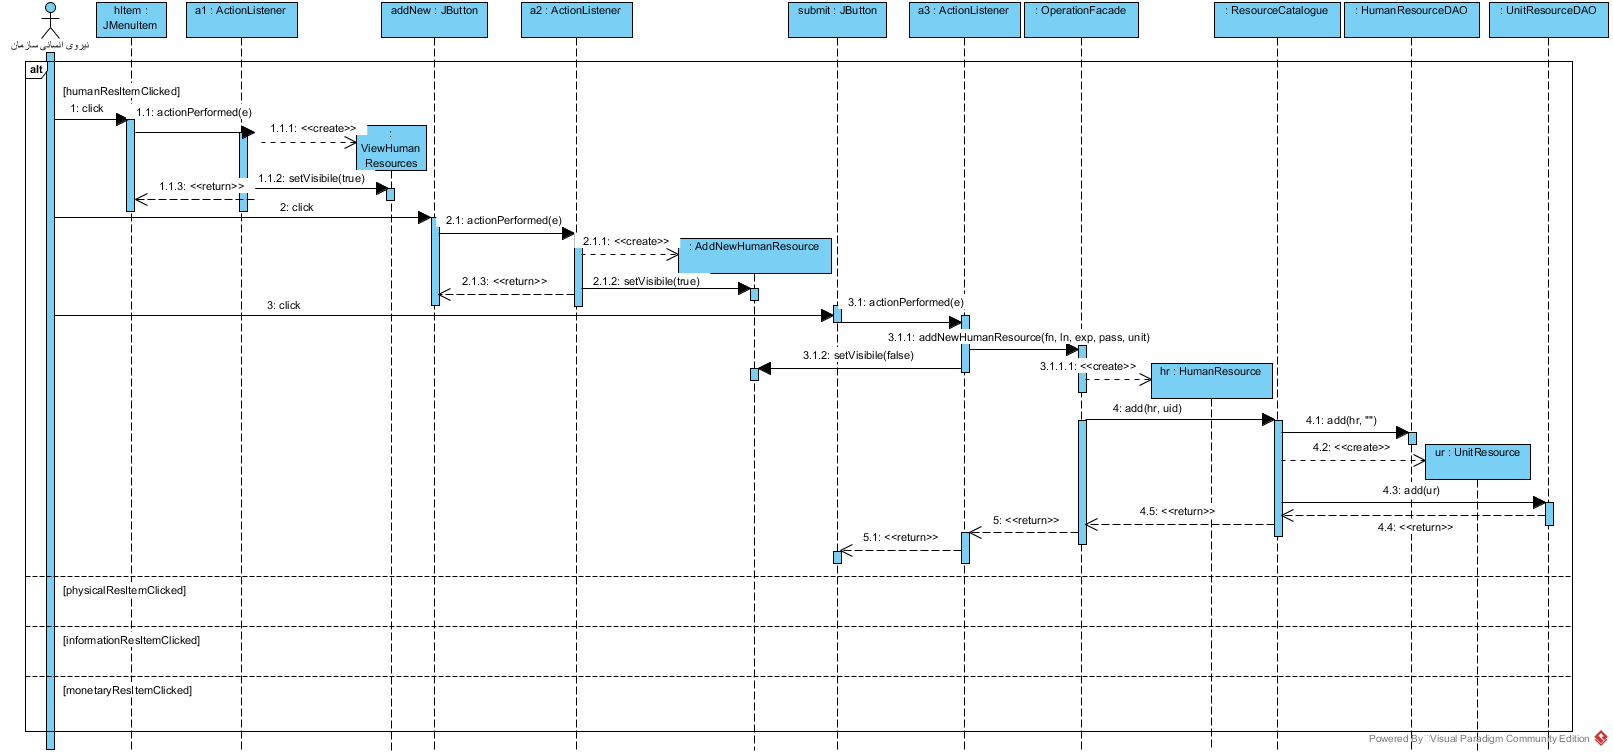
\includegraphics[scale=0.5]{img/sequence-design/AddResourceToUnit_HUMAN}
	\caption{اضافه کردن منبع به واحد سازمان، عملگر منبع انسانی}
\end{figure}
\begin{figure}[H]
	\centering
	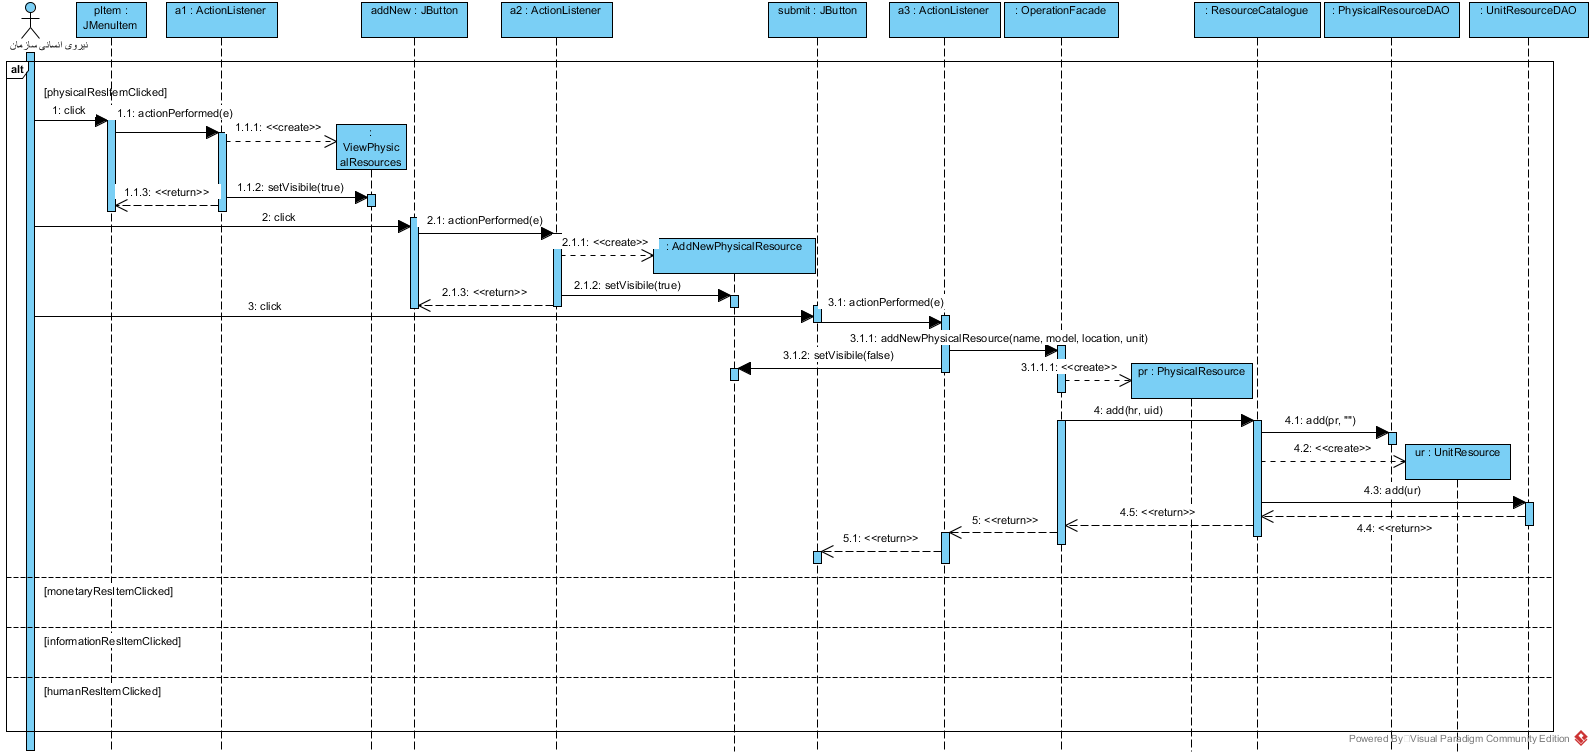
\includegraphics[scale=0.5]{img/sequence-design/AddResourceToUnit_PHYSICAL}
	\caption{اضافه کردن منبع به واحد سازمان، عملگر منبع فیزیکی}
\end{figure}
\begin{figure}[H]
	\centering
	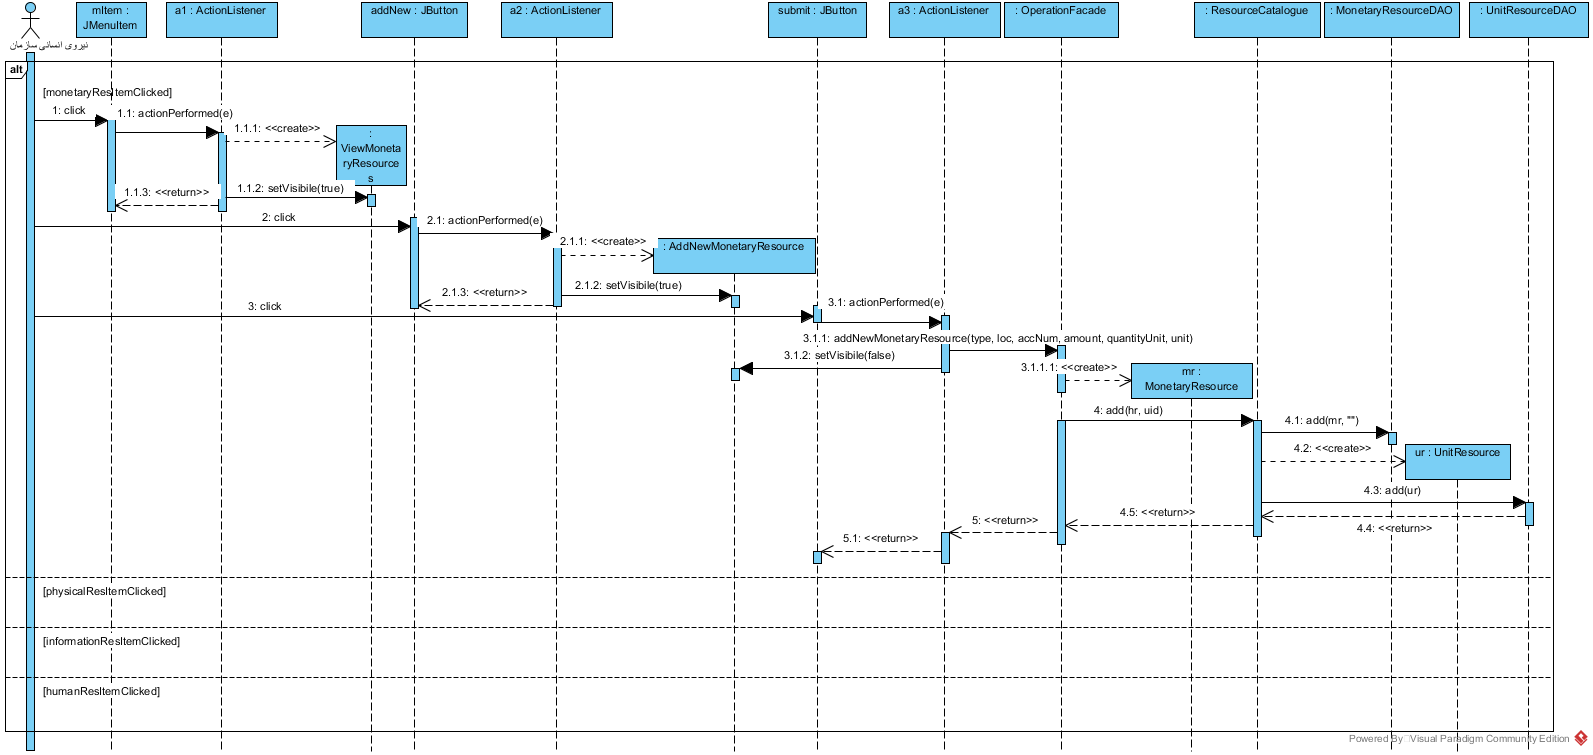
\includegraphics[scale=0.5]{img/sequence-design/AddResourceToUnit_MONETARY}
	\caption{اضافه کردن منبع به واحد سازمان، عملگر منبع مالی}
\end{figure}
\begin{figure}[H]
	\centering
	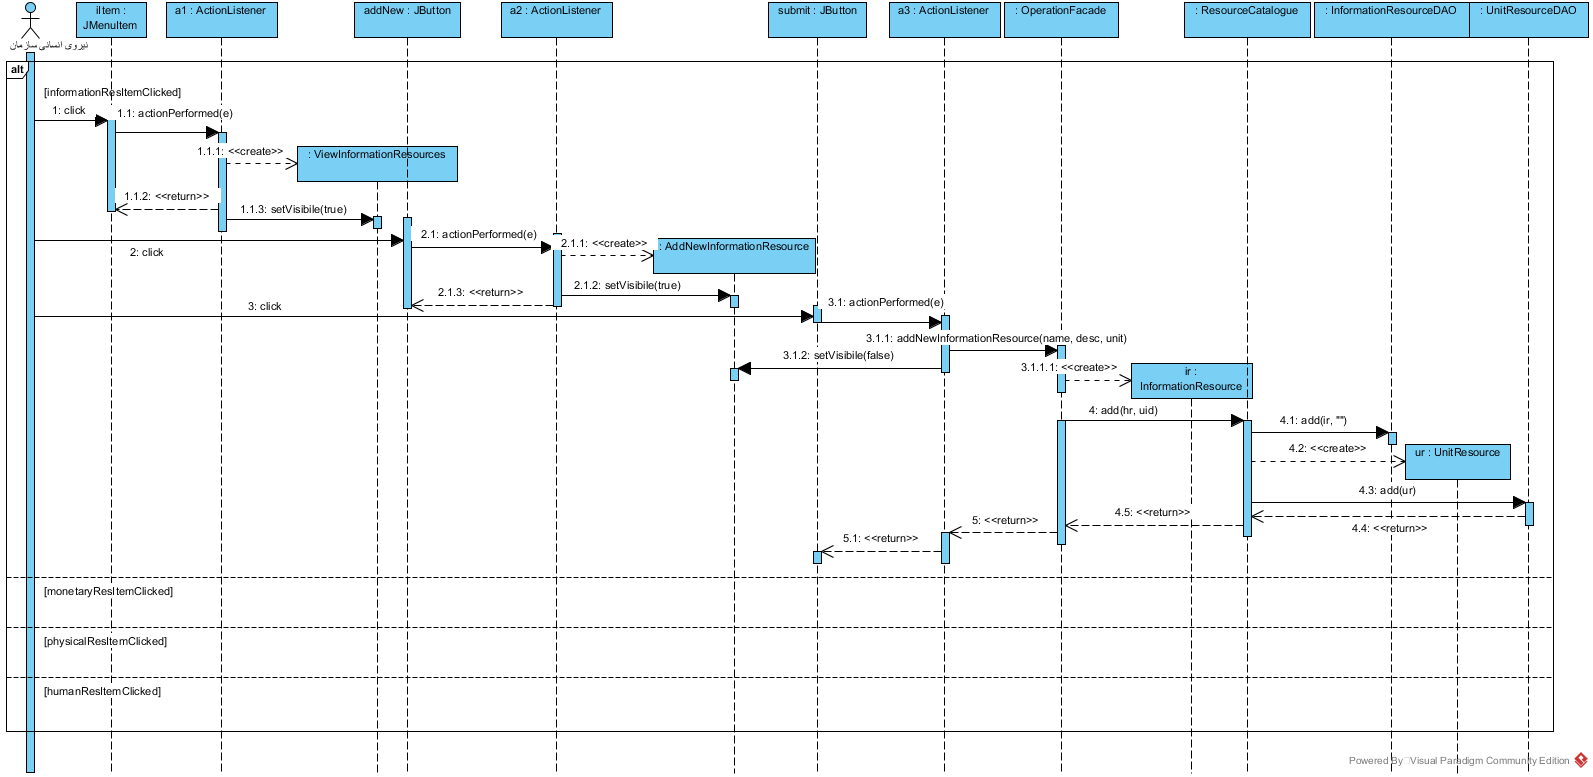
\includegraphics[scale=0.5]{img/sequence-design/AddResourceToUnit_INFORMATION}
	\caption{اضافه کردن منبع به واحد سازمان، عملگر منبع اطلاعاتی}
\end{figure}

\begin{figure}[H]
	\centering
	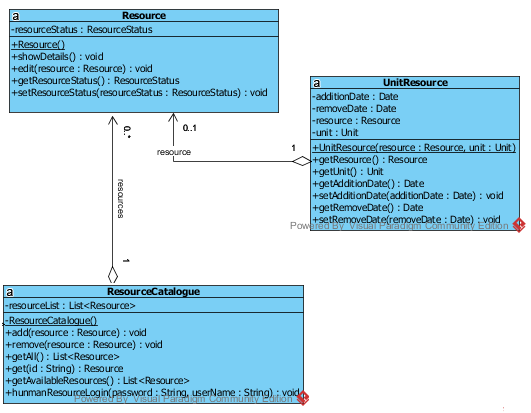
\includegraphics[scale=0.9]{img/sequence-design/AddResourceToUnitC}
	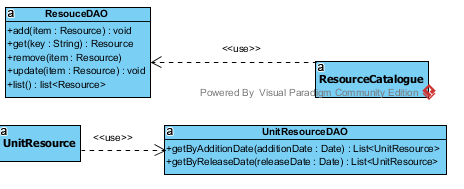
\includegraphics[scale=0.9]{img/sequence-design/AddResourceToUnitD}	
	\caption{اضافه کردن منبع به واحد سازمان}
\end{figure}


\section{افزودن واحد به سازمان}
\begin{figure}[H]
	\centering
	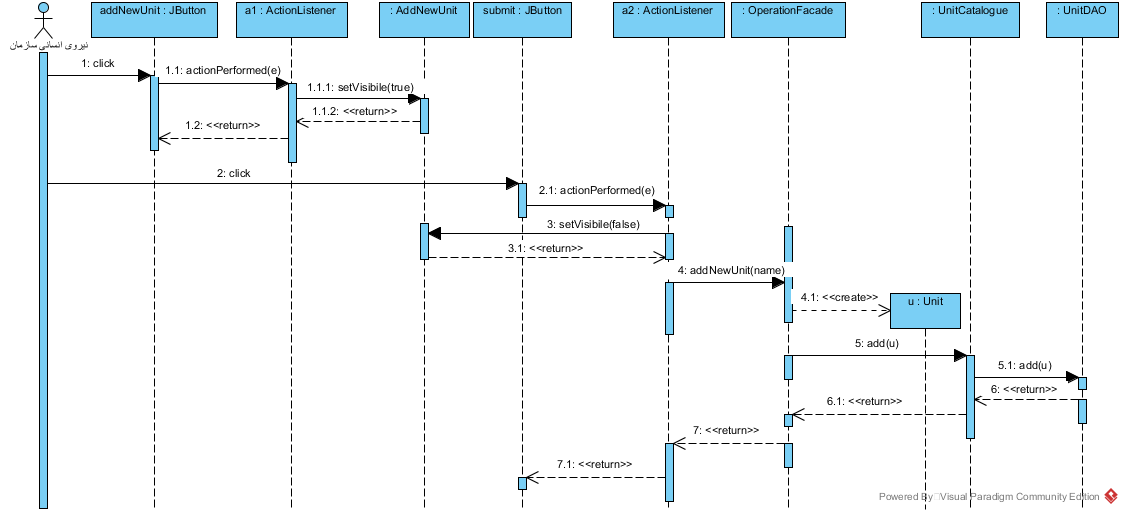
\includegraphics[scale=0.7]{img/sequence-design/AddUnitToOrganization}
	\caption{افزودن واحد به سازمان}
\end{figure}
\begin{figure}[H]
	\centering
	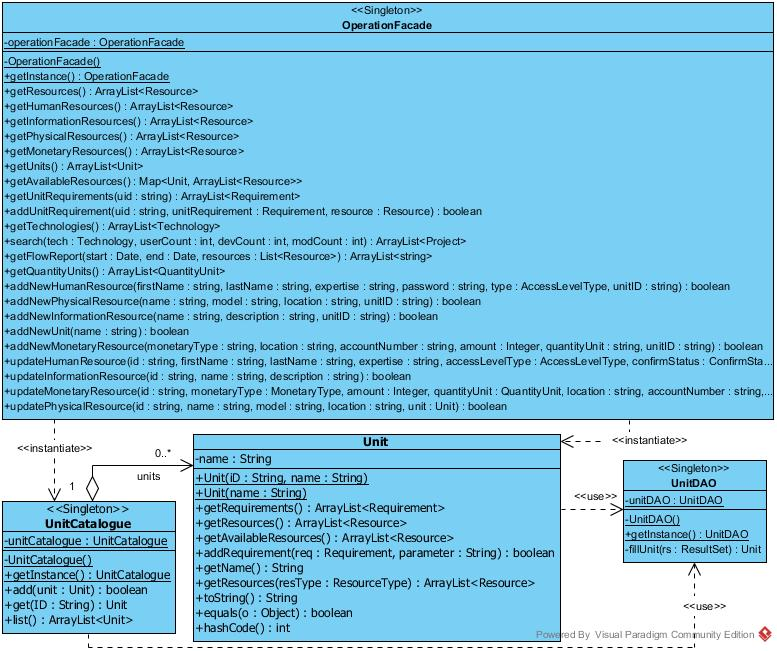
\includegraphics[scale=0.6]{img/sequence-design/AddUnitToOrganizationC}
	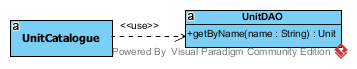
\includegraphics[scale=0.6]{img/sequence-design/AddUnitToOrganizationD}
	\caption{افزودن واحد به سازمان}
\end{figure}


\end{landscape}
\begin{landscape}
\section{رفع نیازمندی پروژه}
\begin{figure}[H]
	\centering
	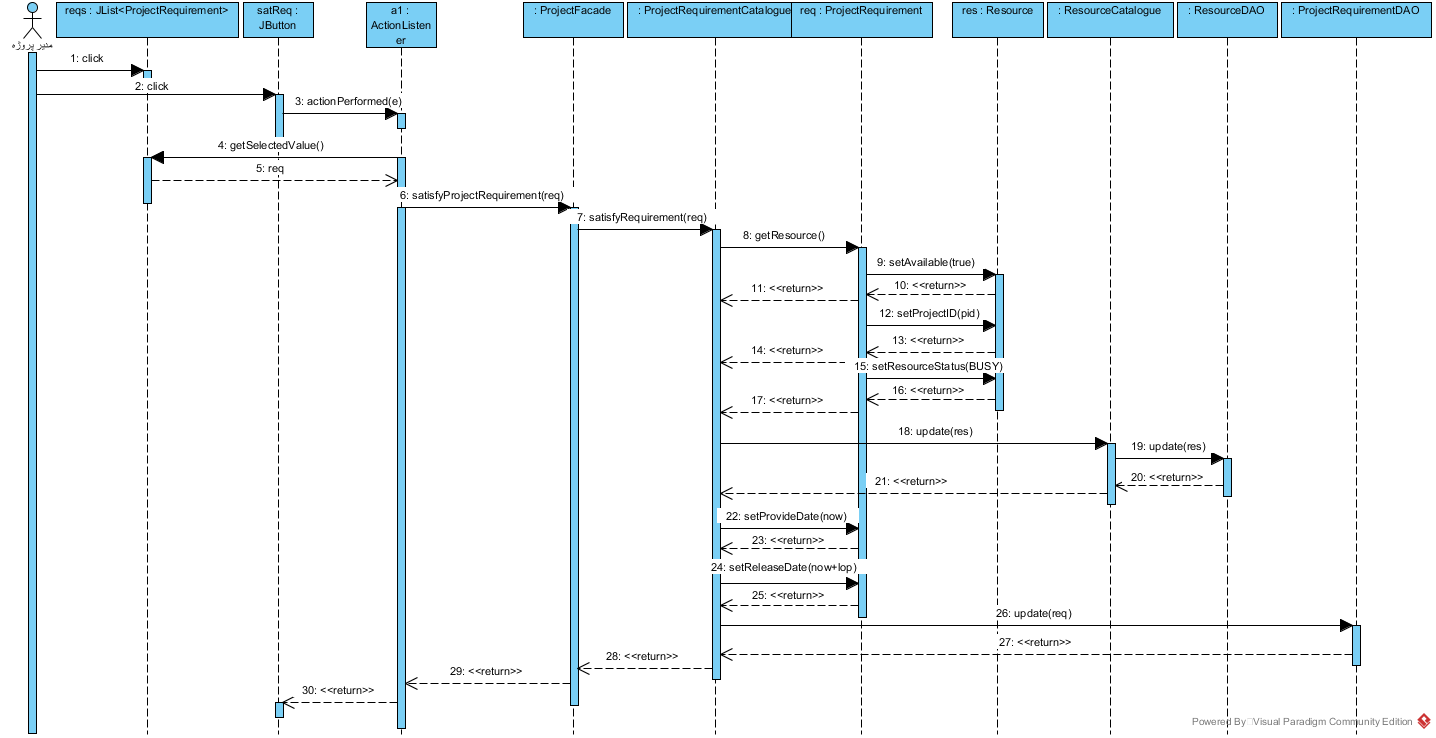
\includegraphics[scale=0.5]{img/sequence-design/SatisfyResourceOfProject}
	\caption{رفع نیازمندی پروژه}
\end{figure}
%\begin{figure}[H]
%	\centering
%	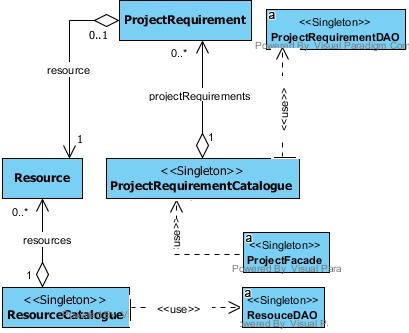
\includegraphics[scale=0.7]{img/sequence-design/SatisfyResourceOfProjectC}
%	\includegraphics[scale=0.7]{img/sequence-design/SatisfyResourceOfProjectD}
%	\caption{رفع نیازمندی پروژه}
%\end{figure}
\end{landscape}

\section{تعیین سطح دسترسی کاربر دیگر}
\begin{figure}[H]
	\centering
	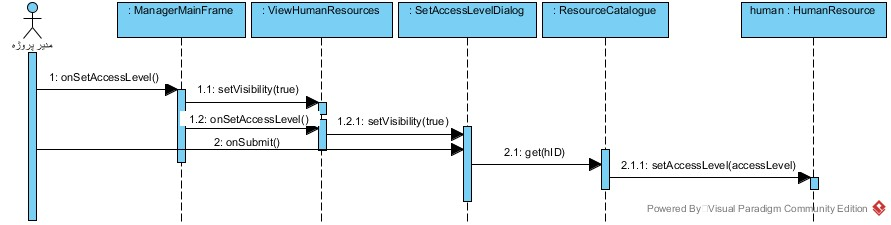
\includegraphics[scale=0.55]{img/sequence-design/SetUserAccessLevel}
	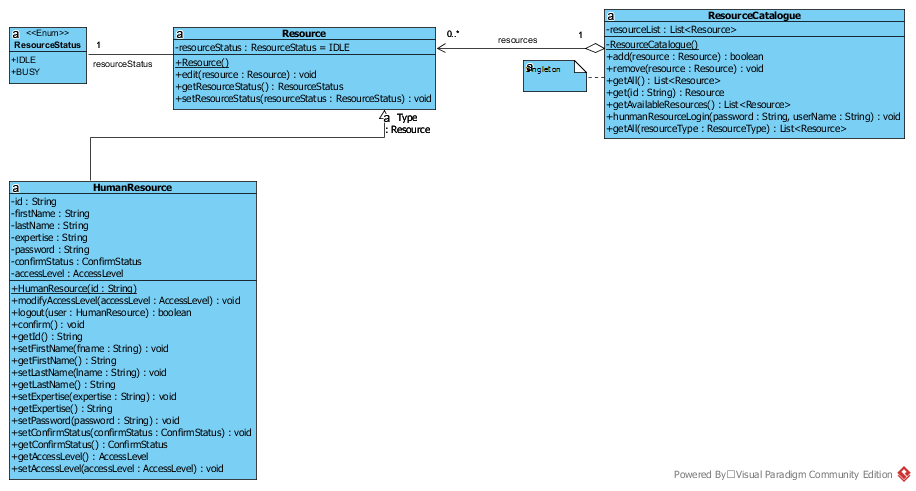
\includegraphics[scale=0.6]{img/sequence-design/SetUserAccessLevelC}
	\caption{تعیین سطح دسترسی کاربر دیگر}
\end{figure}


\section{تعیین عملیات مجاز یک سطح دسترسی}
\begin{figure}[H]
	\centering
	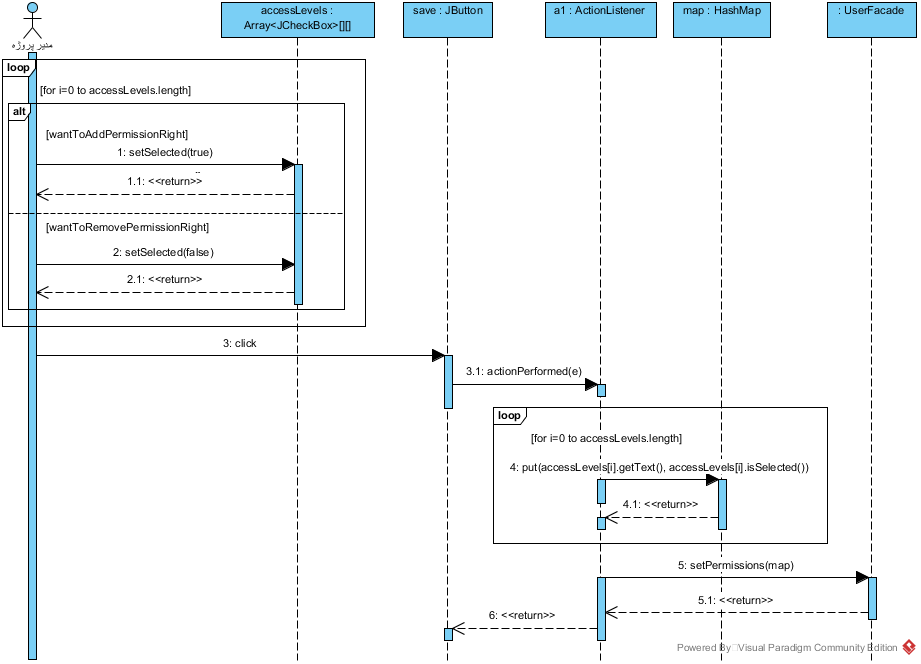
\includegraphics[scale=0.7]{img/sequence-design/SetPermissions}
	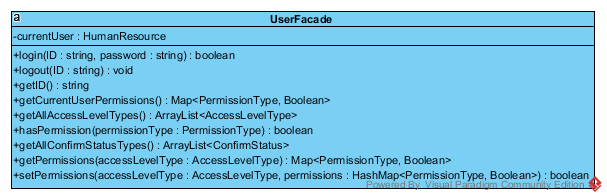
\includegraphics[scale=0.8]{img/sequence-design/SetPermissionsC}
	\caption{تعیین عملیات مجاز یک سطح دسترسی}
\end{figure}


\section{تغییر سطح دسترسی کاربر دیگر}
\begin{figure}[H]
	\centering
	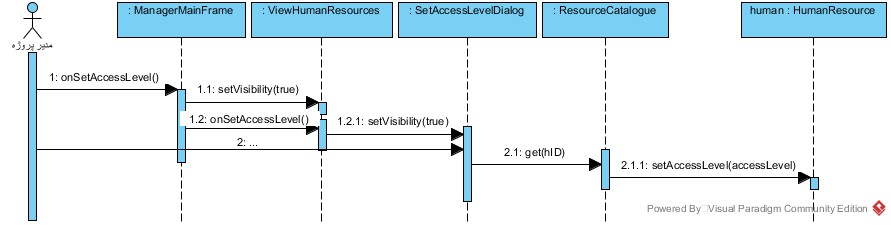
\includegraphics[scale=0.59]{img/sequence-design/ChangeAccessLevel}
	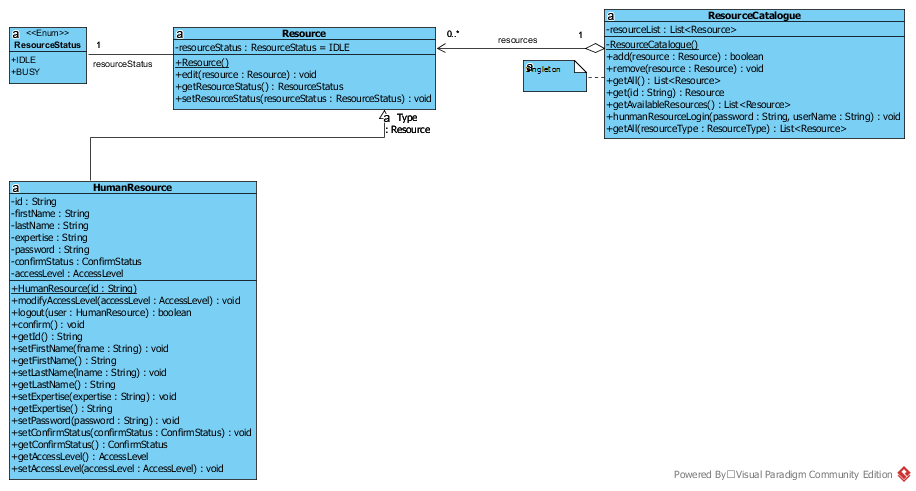
\includegraphics[scale=0.7]{img/sequence-design/ChangeAccessLevelC}
	\caption{تغییر سطح دسترسی کاربر دیگر}
\end{figure}

\begin{landscape}
\section{تغییر مشخصات یک منبع}
این نمودار توالی به علت کلاس‌های زیادی که در آن درگیر هستند، در چهار تصویر و به این صورت در مستند آورده شده که در هر تصویر، تنها یک operand به صورت کامل نشان داده شده است. نکته‌ی دیگر اینکه در این چهار operand از عملگر ref استفاده شده است. اما به علت محدودیت فضا، خطوط زندگی (Lifeline) این رخدادهای تعاملی نشان داده نشده است.
\begin{figure}[H]
	\centering
	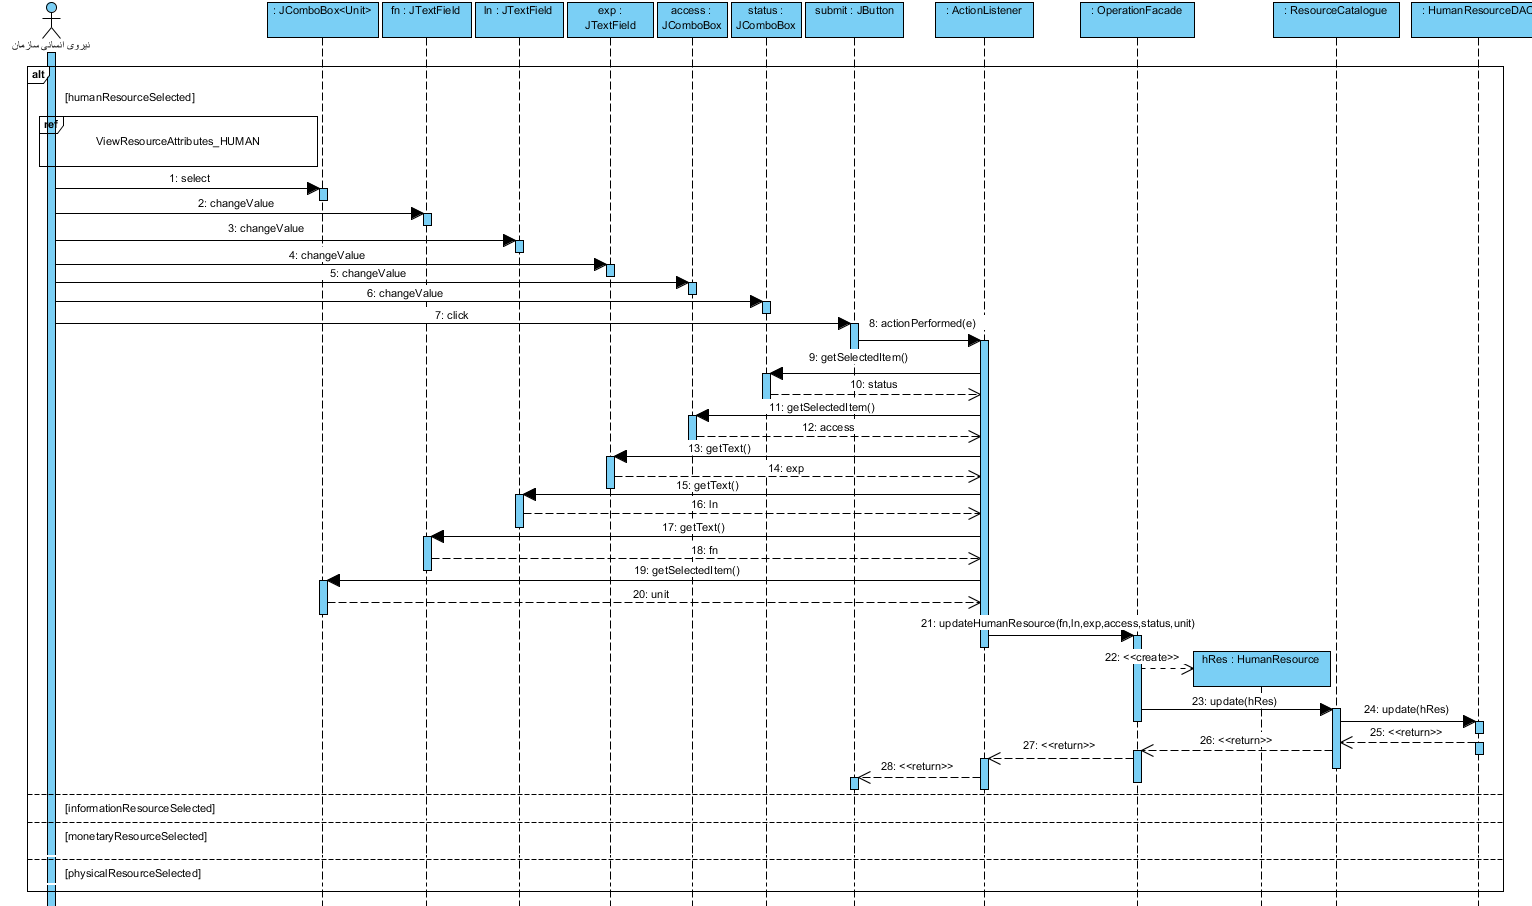
\includegraphics[scale=0.5]{img/sequence-design/EditResourceAttributes_HUMAN}
	\caption{تغییر مشخصات یک منبع، منبع انسانی}
\end{figure}
\begin{figure}[H]
	\centering
	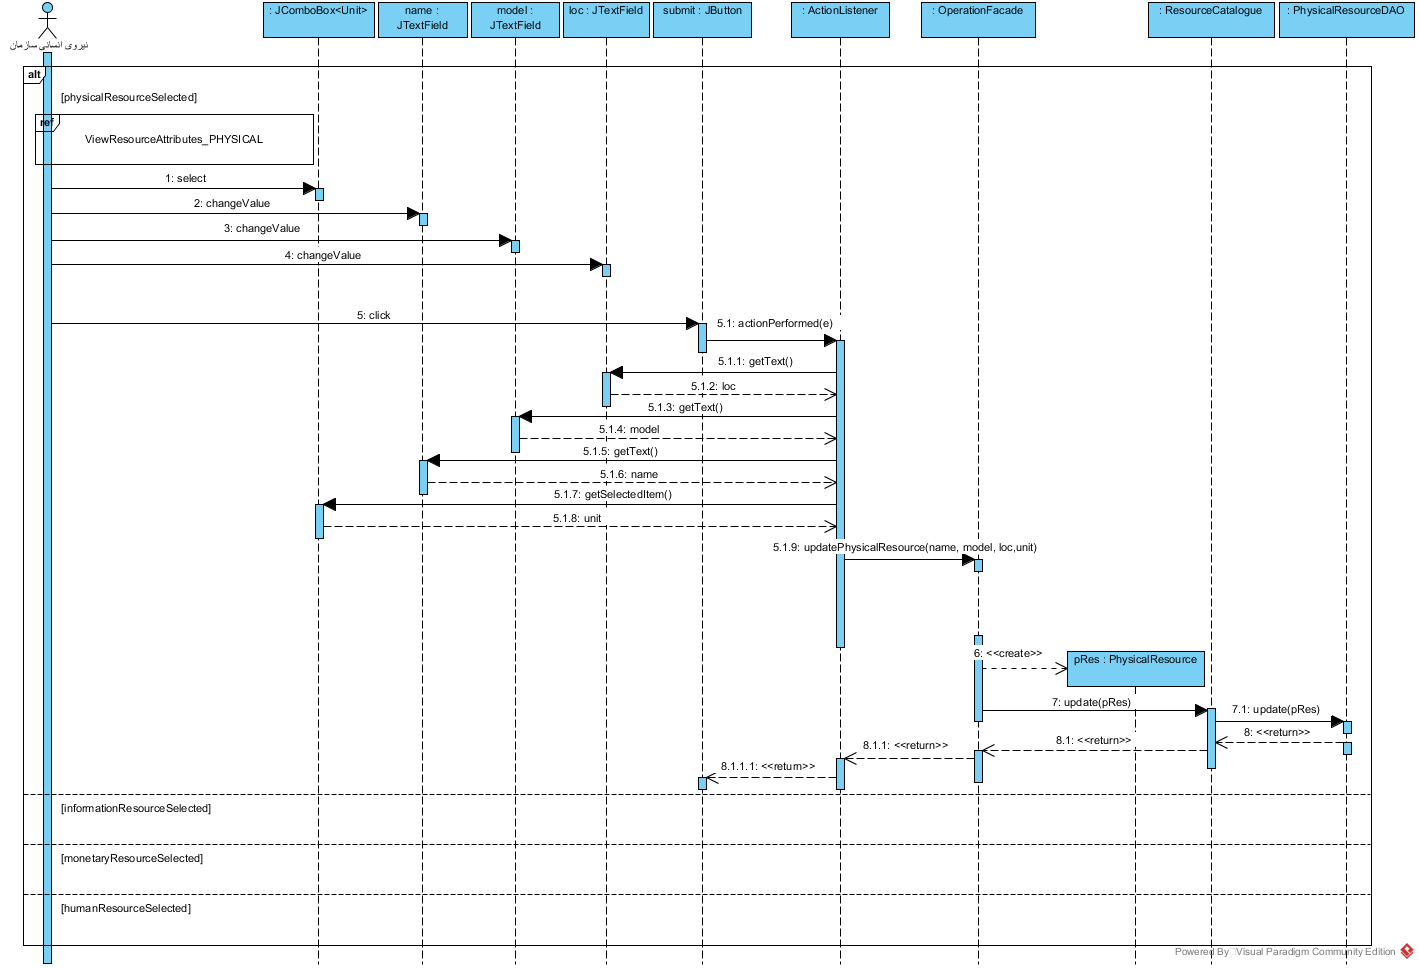
\includegraphics[scale=0.6]{img/sequence-design/EditResourceAttributes_PHYSICAL}
	\caption{تغییر مشخصات یک منبع، منبع فیزیکی}
\end{figure}
\begin{figure}[H]
	\centering
	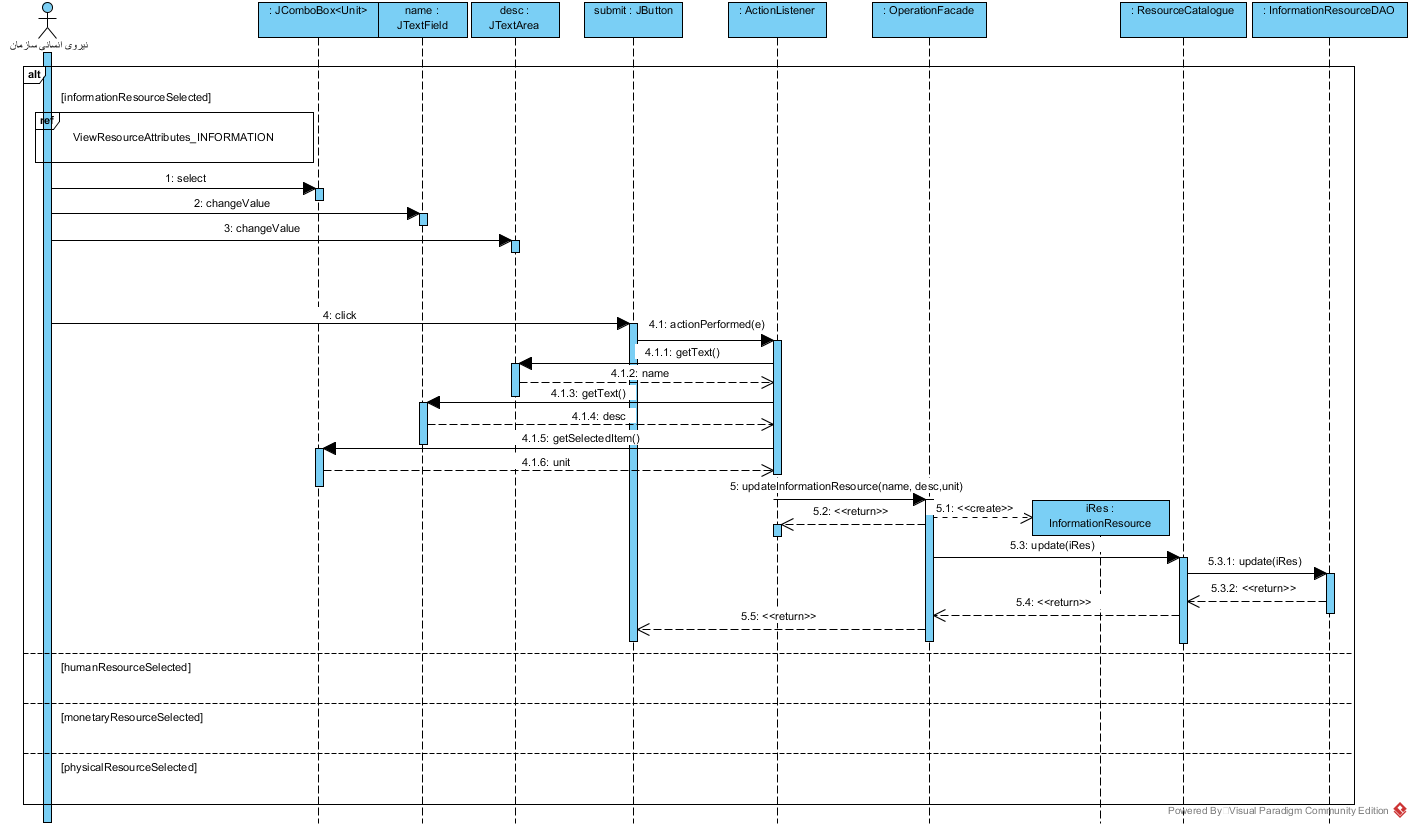
\includegraphics[scale=0.6]{img/sequence-design/EditResourceAttributes_INFORMATION}
	\caption{تغییر مشخصات یک منبع، منبع اطلاعاتی}
\end{figure}
\begin{figure}[H]
	\centering
	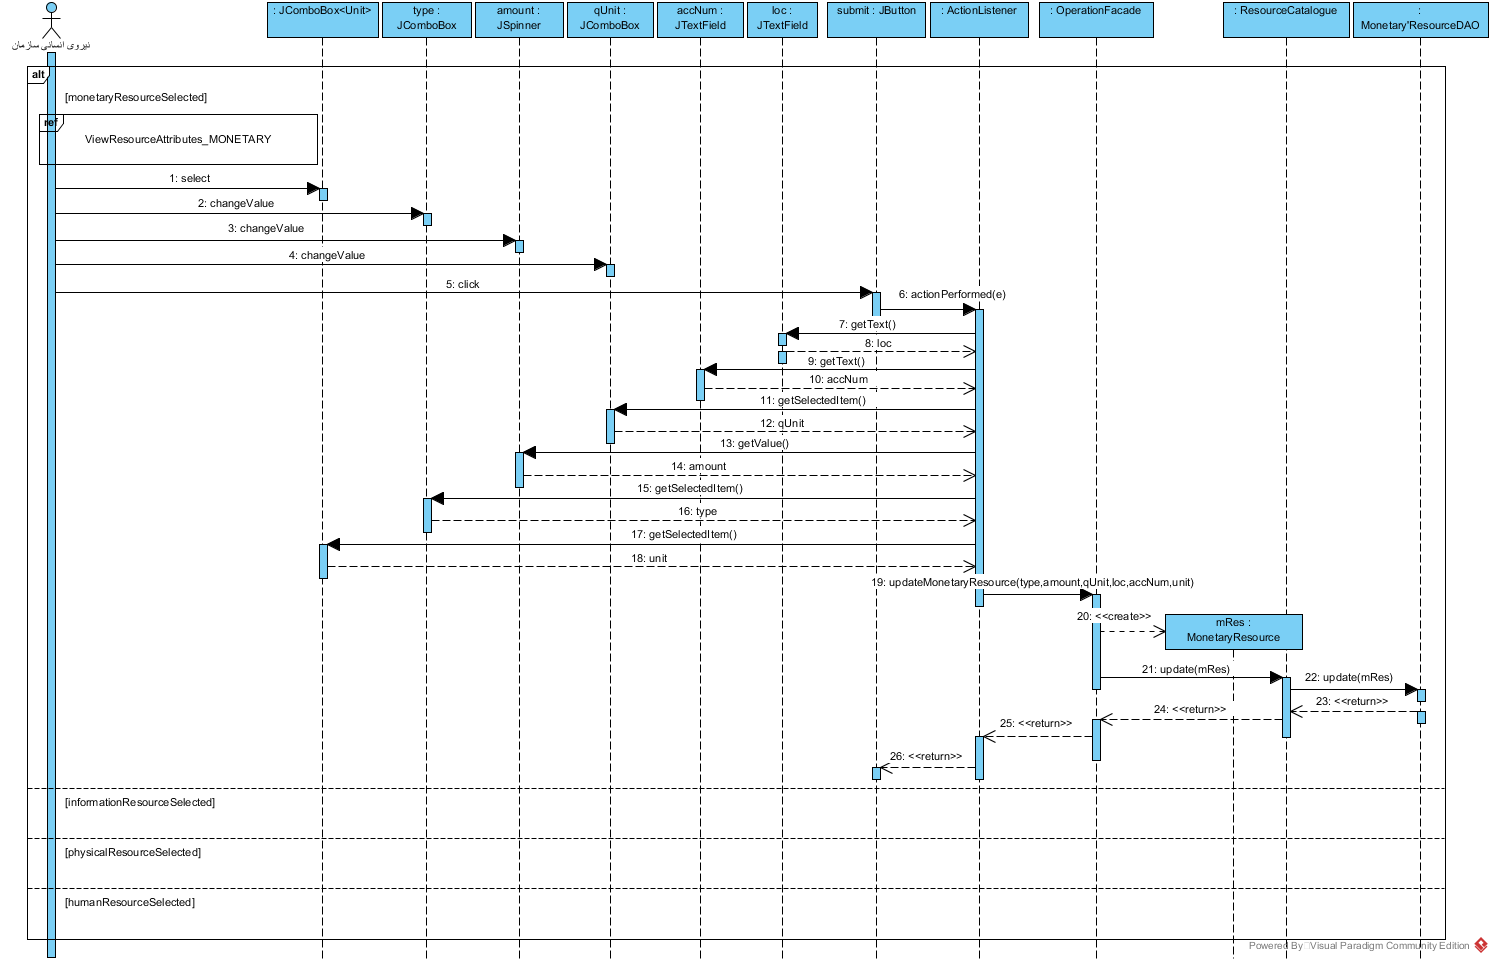
\includegraphics[scale=0.6]{img/sequence-design/EditResourceAttributes_MONETARY}
	\caption{تغییر مشخصات یک منبع، منبع مالی}
\end{figure}

\begin{figure}[H]
	\centering
	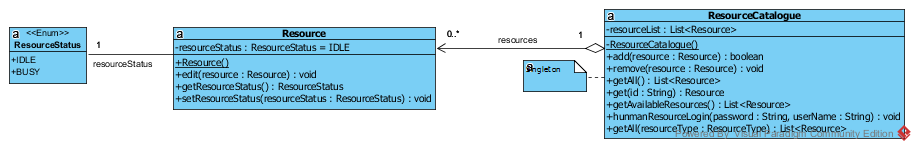
\includegraphics[scale=0.7]{img/sequence-design/EditResourceAttributesC}
	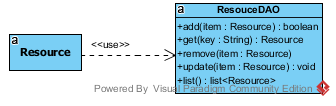
\includegraphics[scale=0.7]{img/sequence-design/EditResourceAttributesD}
	\caption{تغییر مشخصات یک منبع}
\end{figure}

\newpage
\section{ثبت تعداد استفاده‌کنندگان پروژه نرم‌افزاری}
\begin{figure}[H]
	\centering
	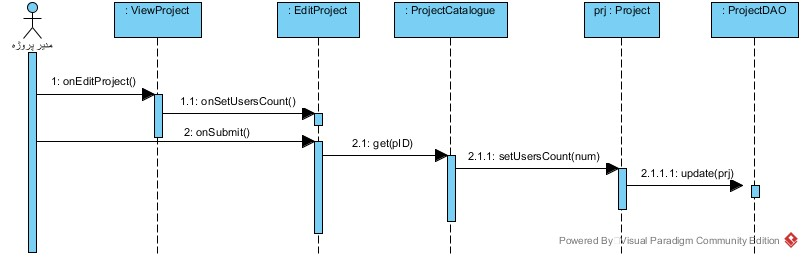
\includegraphics[scale=0.8]{img/sequence-design/AddUsersCount}
\end{figure}
\begin{figure}[H]
	\centering
	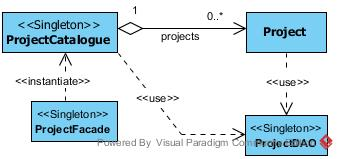
\includegraphics[scale=0.6]{img/sequence-design/AddUsersCountC}
	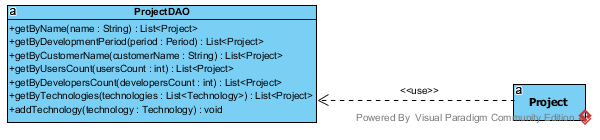
\includegraphics[scale=0.6]{img/sequence-design/AddUsersCountD}
	\caption{ثبت تعداد استفاده‌کنندگان پروژه نرم‌افزاری}
\end{figure}

\section{ثبت تغییر ماژول یک سیستم}
\begin{figure}[H]
	\centering
	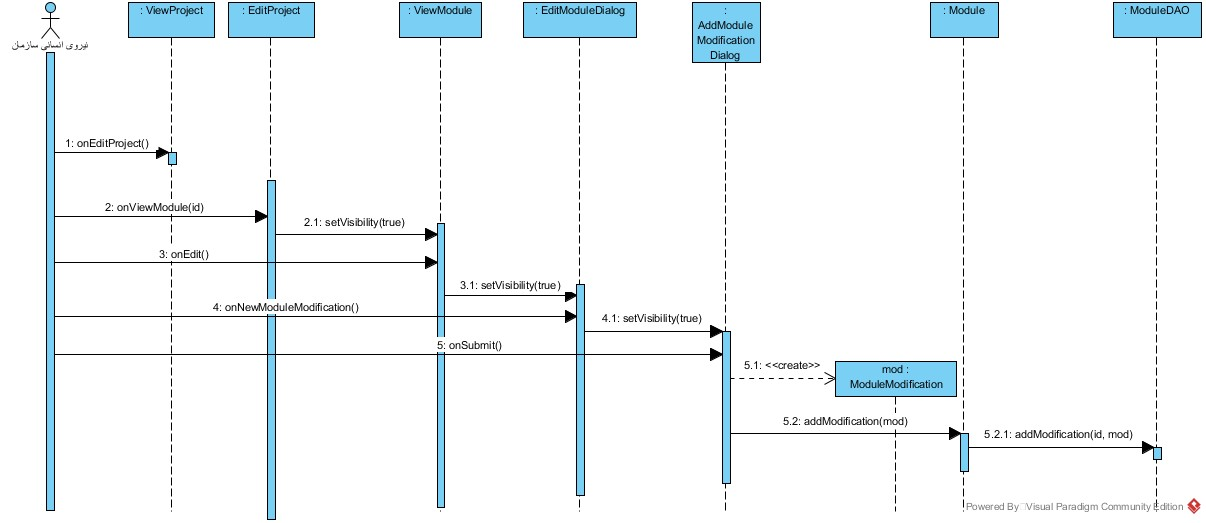
\includegraphics[scale=0.5]{img/sequence-design/AddModuleModification}
	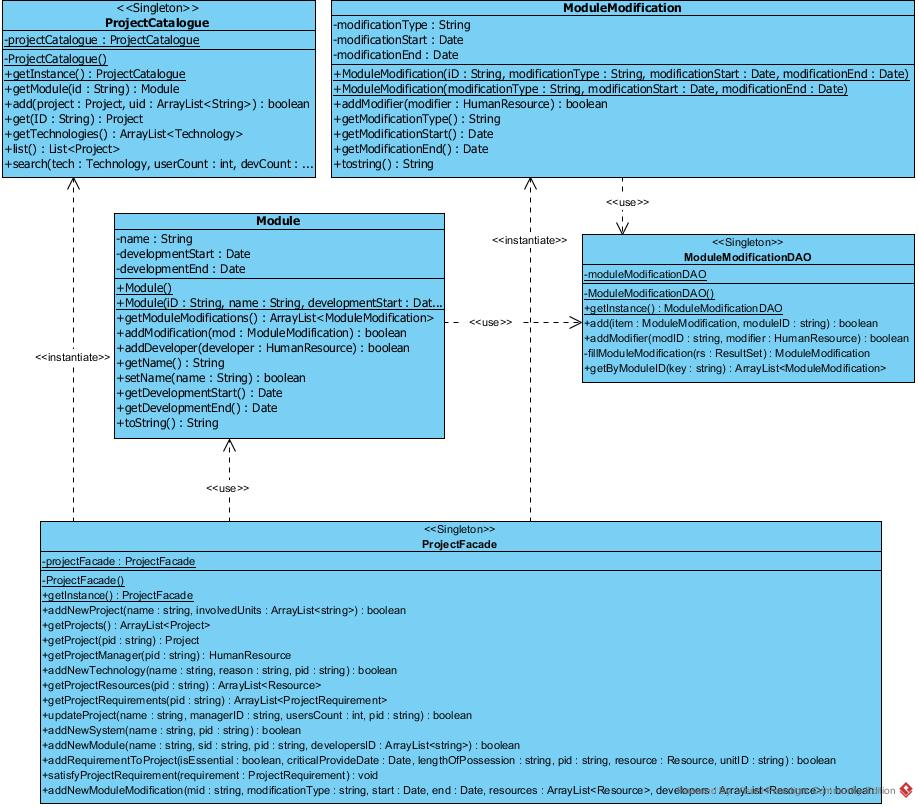
\includegraphics[scale=0.7]{img/sequence-design/AddModuleModificationC}
	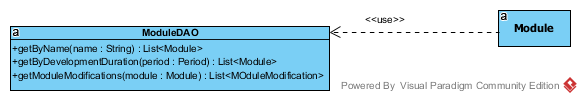
\includegraphics[scale=0.7]{img/sequence-design/AddModuleModificationD}
	\caption{ثبت تغییر ماژول یک سیستم}
\end{figure}

\section{ثبت تکنولوژی مورد استفاده پروژه نرم‌افزاری}
\begin{figure}[H]
	\centering
	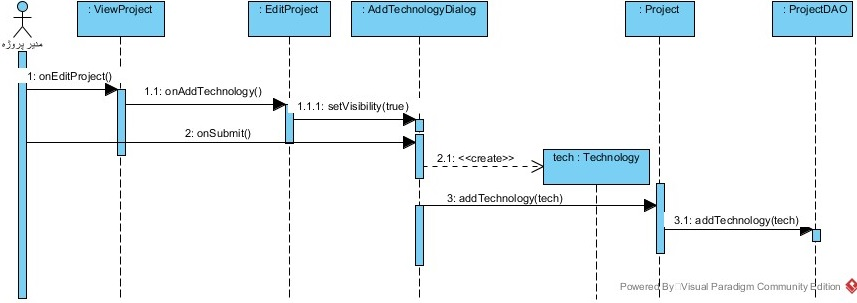
\includegraphics[scale=0.7]{img/sequence-design/AddTechnology}
\end{figure}
\begin{figure}[H]
	\centering
	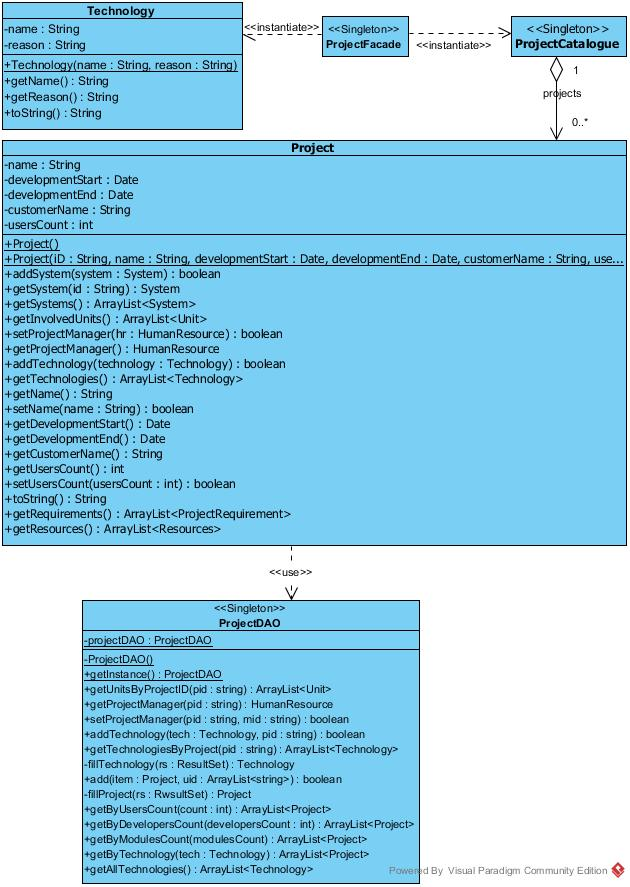
\includegraphics[scale=0.7]{img/sequence-design/AddTechnologyC}
	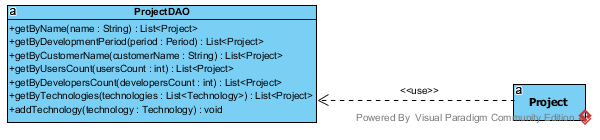
\includegraphics[scale=0.7]{img/sequence-design/AddTechnologyD}
	\caption{ثبت تکنولوژی مورد استفاده پروژه نرم‌افزاری}
\end{figure}

\section{ثبت‌نام در سیستم برنامه‌ریزی}
در این نمودار توالی از عملگر ref استفاده شده است. اما به علت محدودیت فضا، خطوط زندگی (Lifeline) این رخدادهای تعاملی نشان داده نشده است.
\begin{figure}[H]
	\centering
	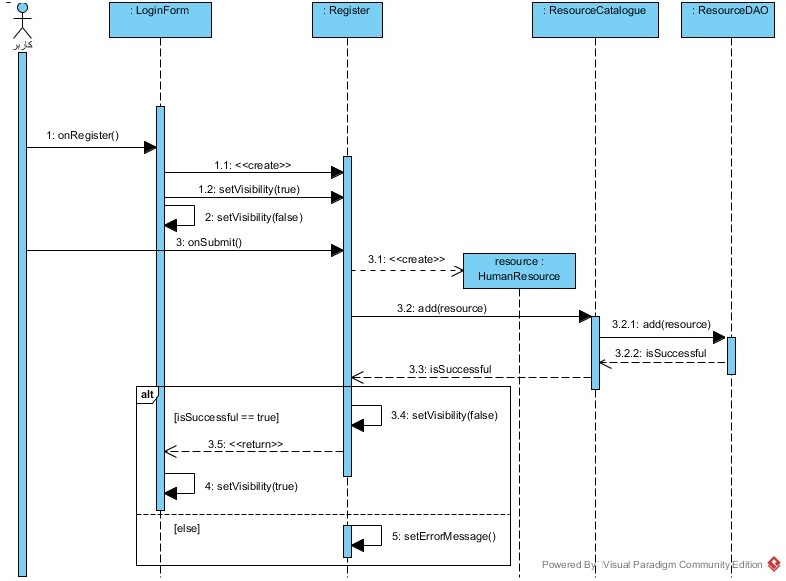
\includegraphics[scale=0.6]{img/sequence-design/SignUp}
\end{figure}
\begin{figure}[H]
	\centering
	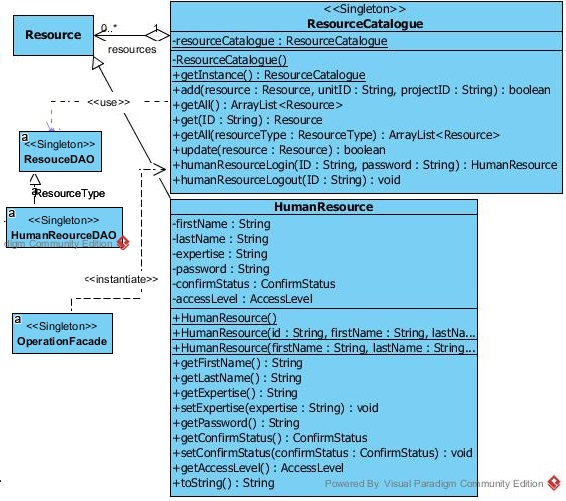
\includegraphics[scale=0.7]{img/sequence-design/SignUpC}
	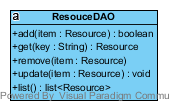
\includegraphics[scale=0.7]{img/sequence-design/SignUpD}
	\caption{ثبت نام در سیستم برنامه ریزی}
\end{figure}
\end{landscape}

\begin{landscape}
\section{ثبت نیازمندی کنونی واحد سازمان}
این نمودار توالی به علت کلاس‌های زیادی که در آن درگیر هستند، در چهار تصویر و به این صورت در مستند آورده شده که در هر تصویر، تنها یک operand به صورت کامل نشان داده شده است.
\begin{figure}[H]
	\centering
	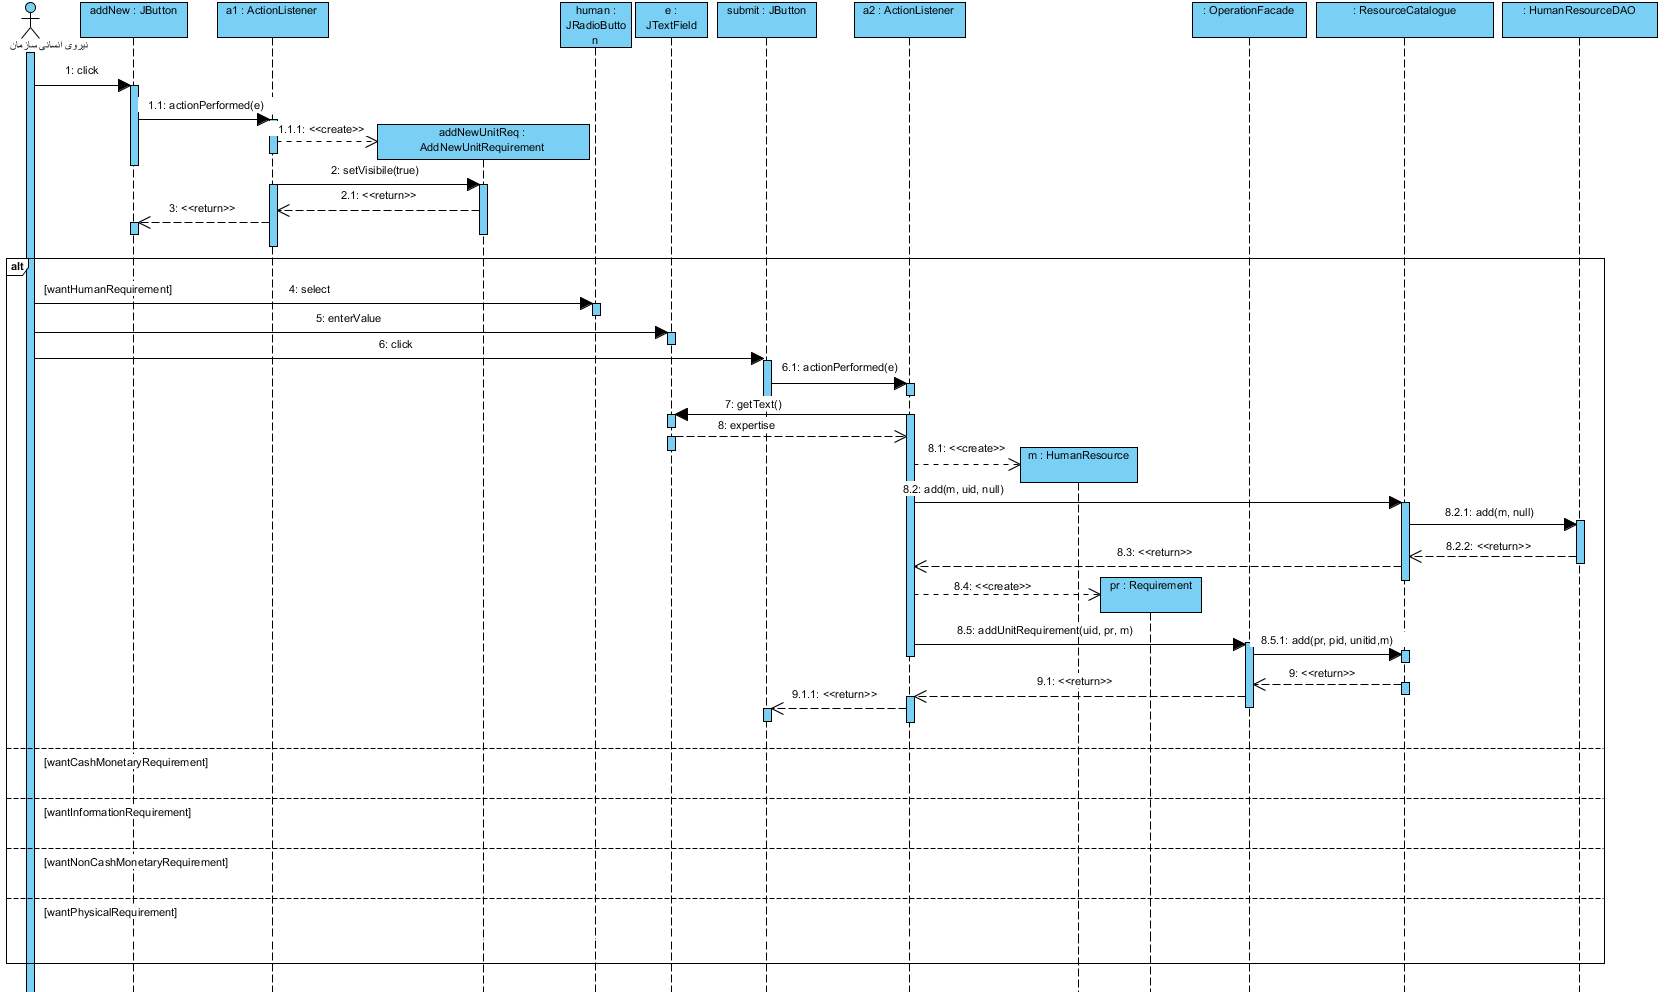
\includegraphics[scale=0.5]{img/sequence-design/AddRequirementToUnit_HUMAN}
	\caption{ثبت نیازمندی کنونی واحد سازمان، منبع انسانی}
\end{figure}
\begin{figure}[H]
	\centering
	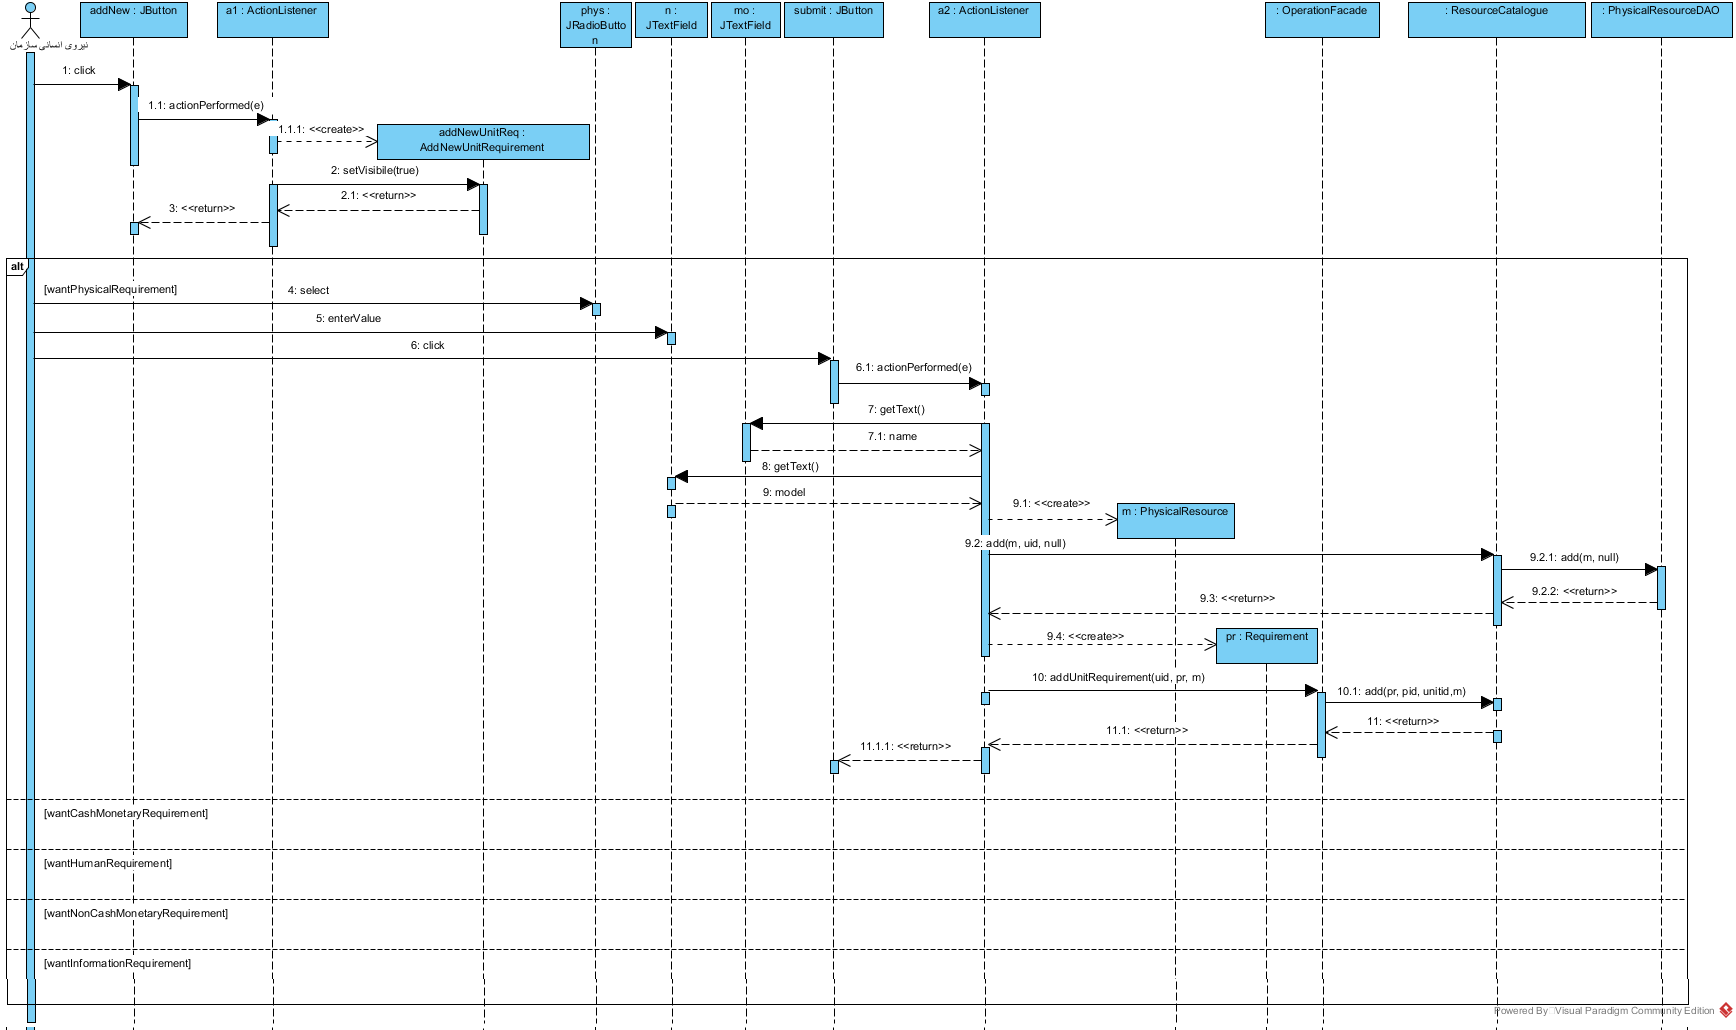
\includegraphics[scale=0.5]{img/sequence-design/AddRequirementToUnit_PHYSICAL}
	\caption{ثبت نیازمندی کنونی واحد سازمان، منبع فیزیکی}
\end{figure}
\begin{figure}[H]
	\centering
	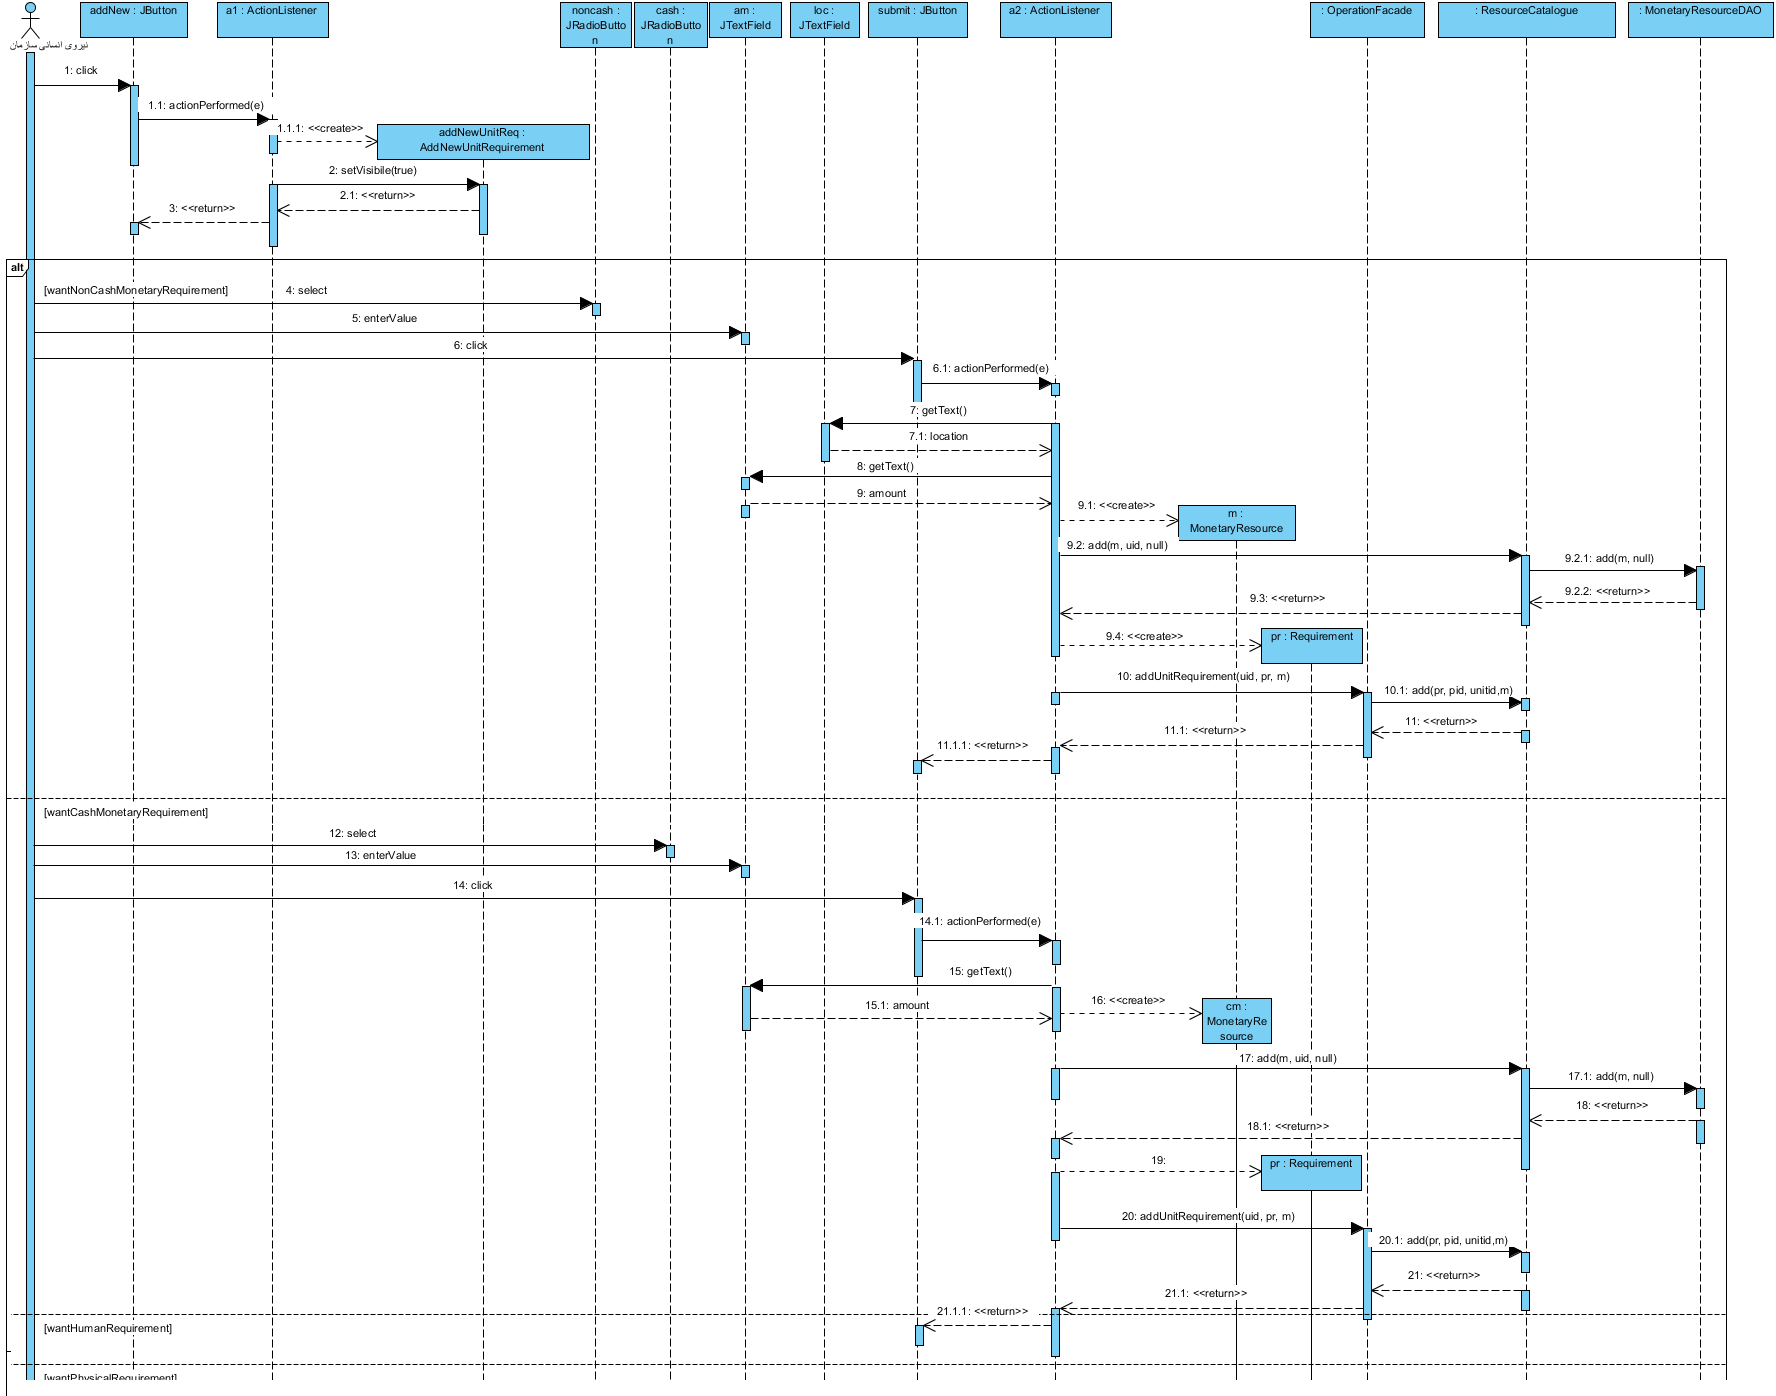
\includegraphics[scale=0.45]{img/sequence-design/AddRequirementToUnit_MONETARY}
	\caption{ثبت نیازمندی کنونی واحد سازمان، منبع مالی}
\end{figure}
\begin{figure}[H]
	\centering
	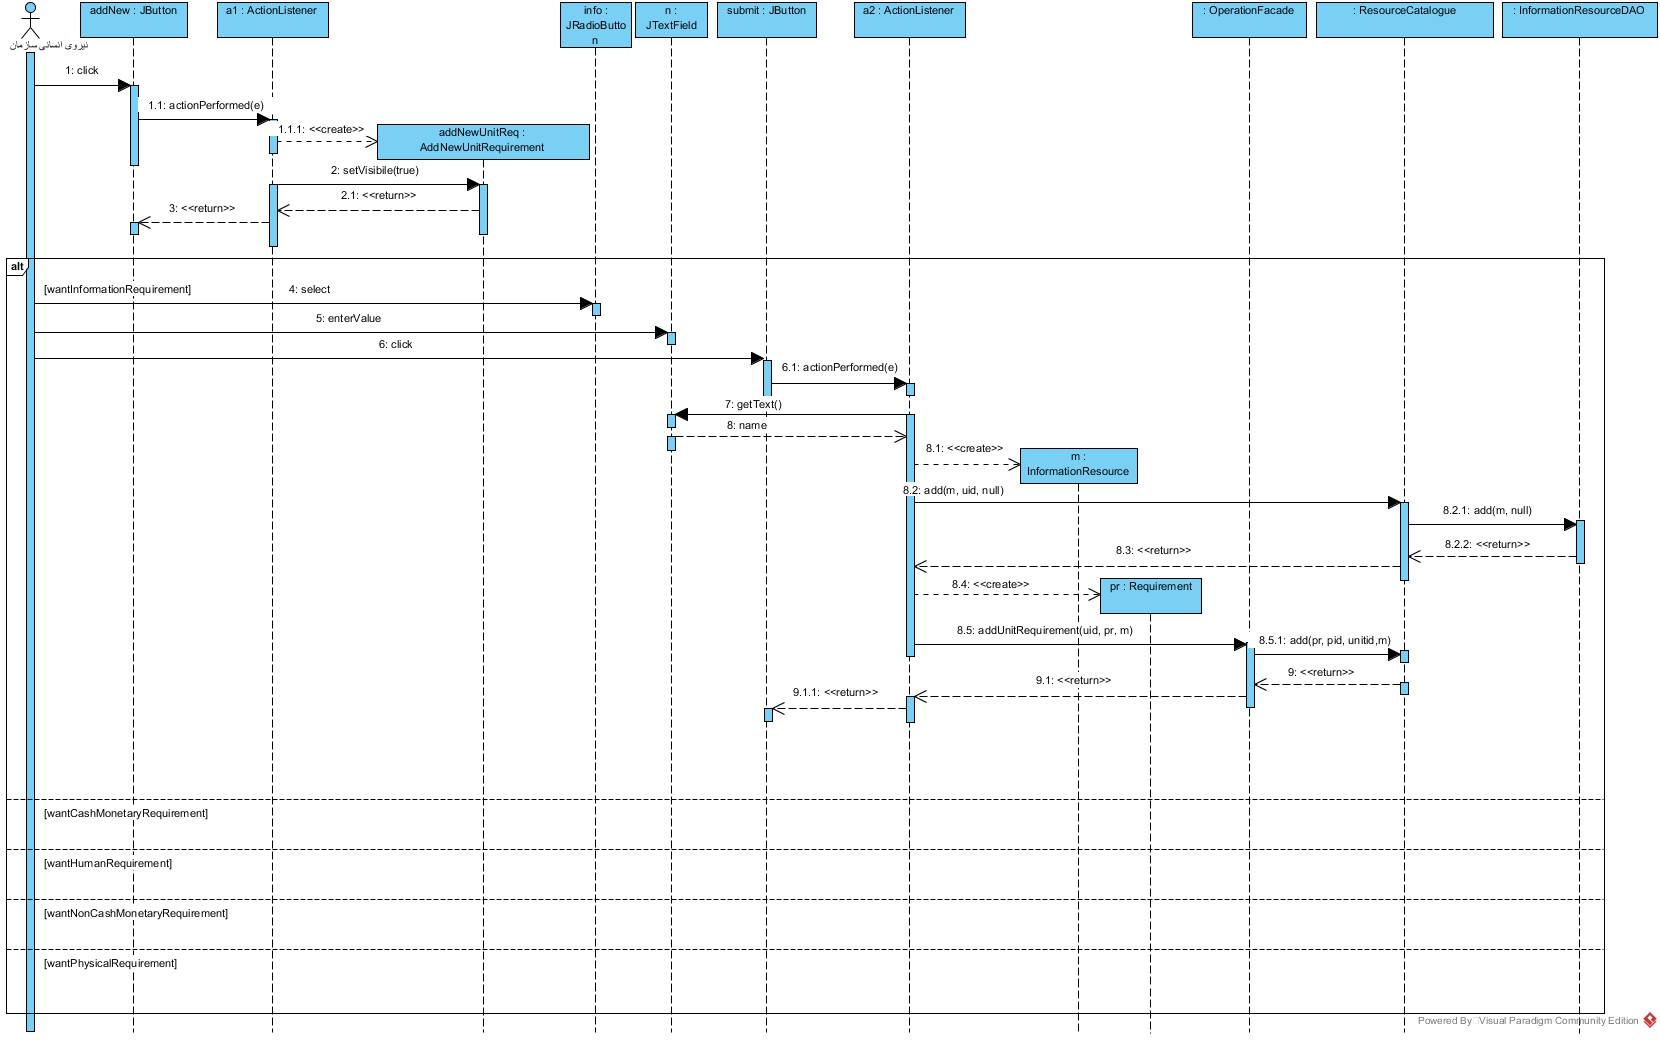
\includegraphics[scale=0.5]{img/sequence-design/AddRequirementToUnit_INFORMATION}
	\caption{ثبت نیازمندی کنونی واحد سازمان، منبع اطلاعاتی}
\end{figure}

\begin{figure}[H]
	\centering
	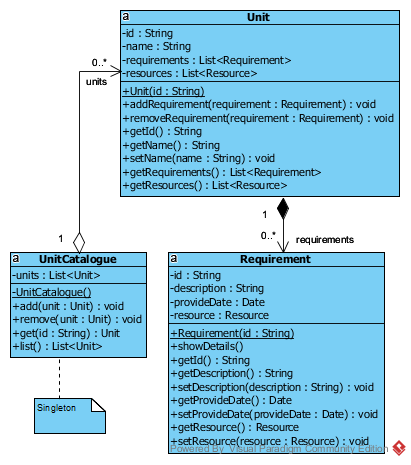
\includegraphics[scale=0.7]{img/sequence-design/AddRequirementToUnitC}
	\includegraphics[scale=0.7]{img/sequence-design/AddRequirementToUnitD}
	\caption{ثبت نیازمندی کنونی واحد سازمان}
\end{figure}


\newpage
\section{اضافه کردن نیازمندی به پروژه}
این نمودار توالی به علت کلاس‌های زیادی که در آن درگیر هستند، در چهار تصویر و به این صورت در مستند آورده شده که در هر تصویر، تنها یک operand به صورت کامل نشان داده شده است.
\begin{figure}[H]
	\centering
	\includegraphics[scale=0.5]{img/sequence-design/AddRequirementToProject_HUMAN}
	\caption{اضافه کردن نیازمندی به پروژه، منبع انسانی}
\end{figure}
\begin{figure}[H]
	\centering
	\includegraphics[scale=0.5]{img/sequence-design/AddRequirementToProject_PHYSICAL}
	\caption{اضافه کردن نیازمندی به پروژه، منبع فیزیکی}
\end{figure}
\begin{figure}[H]
	\centering
	\includegraphics[scale=0.4]{img/sequence-design/AddRequirementToProject_MONETARY}
	\caption{اضافه کردن نیازمندی به پروژه، منبع مالی}
\end{figure}
\begin{figure}[H]
	\centering
	\includegraphics[scale=0.5]{img/sequence-design/AddRequirementToProject_INFORMATION}
	\caption{اضافه کردن نیازمندی به پروژه، منبع اطلاعاتی}
\end{figure}

\begin{figure}[H]
	\centering
	\includegraphics[scale=0.7]{img/sequence-design/AddRequirementToProjectC}
	\includegraphics[scale=0.7]{img/sequence-design/AddRequirementToProjectD}
	\caption{اضافه کردن نیازمندی به پروژه}
\end{figure}

\section{جستجو در پروژه‌ها برای تخمین منبع}
\begin{figure}[H]
	\centering
	\includegraphics[scale=0.6]{img/sequence-design/SearchInProjects}
	\includegraphics[scale=0.7]{img/sequence-design/SearchInProjectsC}
	\caption{جستجو در پروژه ها برای تخمین منبع}
\end{figure}

\section{جستجو در پروژه‌ها برای یافتن نیازمندی‌های ضروری}
\begin{figure}[H]
	\centering
	\includegraphics[scale=0.55]{img/sequence-design/SearchForEssentialRequirements}
	\includegraphics[scale=0.55]{img/sequence-design/SearchForEssentialRequirementsC}
	\caption{جستجو در پروژه‌ها برای یافتن نیازمندی‌های ضروری}
\end{figure}


\section{خروج از سیستم}
\begin{figure}[H]
	\centering
	\includegraphics[scale=0.8]{img/sequence-design/SignOut}
	\caption{خروج از سیستم}
\end{figure}


\section{دریافت گزارش جریان چرخشی مصرف منابع موجود}
\begin{figure}[H]
	\centering
	\includegraphics[scale=0.55]{img/sequence-design/UsageFlowReport}
\end{figure}
\begin{figure}[H]
	\centering
	\includegraphics[scale=0.7]{img/sequence-design/UsageFlowReportC}
	\caption{دریافت گزارش جریان چرخشی مصرف منابع موجود}
\end{figure}

\newpage
\section{دریافت گزارش منابع موجود}
\begin{figure}[H]
	\centering
	\includegraphics[scale=0.7]{img/sequence-design/AvailableResourcesReport}
\end{figure}
\begin{figure}[H]
	\centering
	\includegraphics[scale=0.7]{img/sequence-design/AvailableResourcesReportC}
	\caption{دریافت گزارش منابع موجود}
\end{figure}


\section{دریافت گزارش منابع مورد نیاز}
\begin{figure}[H]
	\centering
	\includegraphics[scale=0.6]{img/sequence-design/RequiredResourcesReport}
\end{figure}
\begin{figure}[H]
	\centering
	\includegraphics[scale=0.7]{img/sequence-design/RequiredResourcesReportC}
	\caption{دریافت گزارش منابع مورد نیاز}
\end{figure}

\section{مشاهده پروژه}
\begin{figure}[H]
	\centering
	\includegraphics[scale=0.7]{img/sequence-design/ViewProject}
\end{figure}
\begin{figure}[H]
	\centering
	\includegraphics[scale=0.8]{img/sequence-design/ViewProjectC}
	\caption{مشاهده پروژه}
\end{figure}

\section{مشاهده فهرست پروژه‌ها}
\begin{figure}[H]
	\centering
	\includegraphics[scale=0.8]{img/sequence-design/ViewListOfProjects}
	\includegraphics[scale=0.9]{img/sequence-design/ViewListOfProjectsC}
	\caption{مشاهده فهرست پروژه‌ها}
\end{figure}


\section{مشاهده فهرست منابع یک واحد}
\begin{figure}[H]
	\centering
	\includegraphics[scale=0.7]{img/sequence-design/ViewListOfResources-1}
	\caption{مشاهده فهرست منابع یک واحد، ادامه در صفحه بعد}
\end{figure}
\begin{figure}[H]
	\centering
	\includegraphics[scale=0.7]{img/sequence-design/ViewListOfResources-2}
	\caption{مشاهده فهرست منابع یک واحد، ادامه از صفحه قبل}
\end{figure}
\begin{figure}[H]
	\centering
	\includegraphics[scale=0.7]{img/sequence-design/ViewListOfResourcesC}
	\caption{مشاهده فهرست منابع یک واحد}
\end{figure}

\section{مشاهده فهرست نیازمندی‌های یک واحد}
\begin{figure}[H]
	\centering
	\includegraphics[scale=0.8]{img/sequence-design/ViewListOfRequirements}
\end{figure}
\begin{figure}[H]
	\centering
	\includegraphics[scale=0.7]{img/sequence-design/ViewListOfRequirementsC}
	\caption{مشاهده فهرست نیازمندی‌های یک واحد}
\end{figure}


\begin{landscape}
\section{مشاهده مشخصات یک منبع}
این نمودار توالی به علت کلاس‌های زیادی که در آن درگیر هستند، در چهار تصویر و به این صورت در مستند آورده شده که در هر تصویر، تنها یک operand به صورت کامل نشان داده شده است.
\begin{figure}[H]
	\centering
	\includegraphics[scale=0.6]{img/sequence-design/ViewResourceAttributes_HUMAN}
	\caption{مشاهده مشخصات یک منبع، منبع انسانی}
\end{figure}
\begin{figure}[H]
	\centering
	\includegraphics[scale=0.8]{img/sequence-design/ViewResourceAttributes_PHYSICAL}
	\caption{مشاهده مشخصات یک منبع، منبع فیزیکی}
\end{figure}
\begin{figure}[H]
	\centering
	\includegraphics[scale=0.8]{img/sequence-design/ViewResourceAttributes_MONETARY}
	\caption{مشاهده مشخصات یک منبع، منبع مالی}
\end{figure}
\begin{figure}[H]
	\centering
	\includegraphics[scale=0.8]{img/sequence-design/ViewResourceAttributes_INFORMATION}
	\caption{مشاهده مشخصات یک منبع، منبع اطلاعاتی}
\end{figure}

\begin{figure}[H]
	\centering
	\includegraphics[scale=0.7]{img/sequence-design/ViewResourceAttributesC}
	\caption{مشاهده مشخصات یک منبع}
\end{figure}
\end{landscape}

\section{ورود به سیستم}
\begin{figure}[H]
	\centering
	\includegraphics[scale=0.65]{img/sequence-design/SignIn}
\end{figure}
\begin{figure}[H]
	\centering
	\includegraphics[scale=0.6]{img/sequence-design/SignInCD}
	\caption{ورود به سیستم}
\end{figure}
\end{landscape}